% DIAGRAM : https://app.diagrams.net/#G1Plt8chIOiykQ_dkGwUgM7g10JzzMdCI_ \\
% ilustrasi gambar : https://www.canva.com/design/DAFNN__rHQg/24fsfugJXtRI3ku2XGhdTg/edit#
Implementasi yang ingin dicapai pada proyek ini adalah terbentuknya sistem untuk mendeteksi manusia dan benda untuk robot \covid. Sistem akan berupa simulasi mengenai proses pembacaan data lingkungan, pemrosesan data, dan luaran hasil deteksi. Semua proses akan dibuat menggunakan bahasa pemrograman \textit{python}. Program yang dibuat diharapkan dapat dengan mudah untuk diimplementasikan dan dikembangkan pada robot \covid. Data lingkungan diperoleh dari gambar denah yang disediakan kemudian diubah menjadi data luaran yang memiliki bentuk yang serupa mungkin dengan data luaran \lidar\ pada umumnya. Proyek ini berfokus untuk mengolah hasil bacaan \lidar\ terhadap lingkungan sekitar dan menampilkan hasil bacaan teridentifikasi sebagai objek manusia atau benda.  

\section{Luaran \textit{Capstone Project} beserta Spesifikasinya}
\label{sec:Luaran_Capstone_Project_beserta_Spesifikasinya}

  Proyek \capstone\ ini bertujuan untuk membuat sistem yang berhasil mendeteksi kaki manusia dari bacaan mentah \lidar\ dan meminimalkan \textit{error} bacaan. Sistem dibuat dari simulasi bacaan \lidar\ hingga menampilkan hasil deteksi. Pendeteksian kaki manusia merupakan masalah yang cukup rumit, namun dalam sistem ini diaplikasikan metode deteksi yang sederhana berbasis regresi. Metode ini tidak memerlukan sensor tambahan lainnya untuk memvisualkan kondisi lingkungan sekitar, sehingga robot yang memiliki \lidar\ 2D sudah dapat mengaplikasikan sistem pendeteksian ini. Modifikasi dan uji coba akan banyak dilakukan pada program agar menghasilkan sistem yang dengan tepat mendeteksi objek dan simulasi semirip mungkin dengan kejadian asli pendeteksian \lidar. Luaran proyek yang dijanjikan pada \textit{capstone} ini dituliskan pada Tabel \ref{tab:Ch06_Contoh_Luaran}.
    
    \begin{longtable}{|L{3cm}|L{4cm}|L{7.8cm}|}
        \caption{Luaran \textit{Capstone Project}} 
        \label{tab:Ch06_Contoh_Luaran}
        \vspace{-0.75em}\\        
        \hline
        \multicolumn{1}{|c|}{\textbf{Jenis Luaran}} & \multicolumn{1}{|c|} {\textbf{Nama}} & \multicolumn{1}{|c|} {\textbf{Penjelasan}} \\ \hline

        \textit{Source Code}
        & \textit{Library} Pembaca Denah Lingkungan
        & Program dalam bentuk \textit{library} untuk membaca gambar denah ruangan. Gambar denah diubah dari gambar berwarna hitam putih menjadi data yang akan diproses \lidar\ sehingga menghasilkan luaran yang dapat diproses sistem. Sumber data lingkungan hanya berupa gambar karena sistem deteksi belum diaplikasikan pada \lidar\ asli yang beroperasi dalam robot. Lingkungan sistem berasal dari gambar yang skala berbagai objeknya akan disesuaikan dengan ukuran lingkungan asli.   
        \\ \hline

        \textit{Source Code}
        & \textit{Library} Pembuat Data \lidar
        & Program dalam bentuk \textit{library} untuk membaca data denah dan membuat data sesuai dengan format luaran \lidar\ asli. Data akan diproses oleh program \lidar\ sehingga menghasilkan luaran yang sesuai dengan spesifikasi \lidar\ untuk nanti digunakan dalam pemrosesan sistem deteksi.  
        \\ \hline
        
        \textit{Source Code}
        & \textit{Library} Deteksi Garis dan Lingkaran
        & Program dalam bentuk \textit{library} untuk mendeteksi bentuk lingkungan dari data \lidar\ dan membedakannya menjadi dua kelompok yaitu berupa kelompok garis dan kelompok lingkaran. Program akan berisi berbagai fungsi matematika yang akan digunakan dalam proses deteksi dan segmentasi data \lidar.
        \\     \hline

        \textit{Source Code}
        & Program Sistem Deteksi dan Klasifikasi
        & Program untuk mengelompokkan segmen garis dan lingkaran menjadi manusia dan non manusia kemudian ditampilkan pada simulasi. Lingkaran-lingkaran yang teridentifikasi sebagai manusia akan diberi bingkai berbentuk  segi empat, sementara untuk non manusia hanya akan ditampilkan bentuk garis atau lingkaran. Program ini juga berisi algoritma utama yang digunakan dalam deteksi yang dapat menjalankan simulasi utuh robot. Program ini menyatukan beberapa \textit{library} yang dibuat pada proyek \capstone\ untuk membuat simulasi pendeteksian manusia pada robot berjalan dalam ruangan. 
        \\     \hline

        Simulasi
        & Simulasi Robot Bergerak 
        & Simulasi sistem deteksi \lidar\ pada robot yang bergerak di dalam suatu denah ruangan menggunakan fitur \textit{pygame}. Robot akan berjalan otomatis melewati berbagai objek dengan posisi diam. 
        \\     \hline
    \end{longtable}   
    
    Tabel \ref*{tab:Ch06_Contoh_Luaran} memperlihatkan luaran \capstone\ terdiri dari dua jenis yaitu \textit{source code} dan simulasi. \textit{Source code} berisi program yang dibedakan menjadi 3 jenis yang digunakan mulai dari pembacaan gambar denah hingga klasifikasi. Komponen-komponen simulasi juga disusun menggunakan \textit{source code} yang dibuat. Luaran \textit{source code} dipisah menjadi empat buah \textit{file} yaitu \textit{file} untuk pembuatan lingkungan, \textit{file} pembuatan sensor, \textit{file} pembuatan fitur-fitur sistem, dan \textit{file} utama seperti yang terlihat pada lampiran. Program deteksi garis dan lingkaran berada dalam \textit{file} pembuatan fitur-fitur sistem sedangkan program klasifikasi berada dalam \textit{file} utama. Hal ini dilakukan untuk mempermudah proses pengeditan, penambahan program, dan diharapkan juga untuk mempermudah program jika akan dipakai dalam proyek lain. Luaran simulasi berupa tampilan yang muncul pada layar komputer. Simulasi ini akan menjalankan proses sistem deteksi pada sebuah robot bergerak di dalam ruangan yang dibuat pada denah.

    Agar produk \textit{capstone} dapat memberikan hasil yang berfungsi dengan baik perlu ditentukan beberapa spesifikasi mengenai detail sistem yang ingin diimplementasikan. Spesifikasi luaran yang akan didesain dapat dilihat pada Tabel \ref{tab:Ch06_Contoh_Spesifikasi_Luaran}.
    
    \begin{longtable}{|c|c|c|L{3.8 cm}|c|}
        \caption{Spesifikasi Luaran} 
        \label{tab:Ch06_Contoh_Spesifikasi_Luaran}
        \vspace{-0.75em}\\
        \hline
        \textbf{No.} & \textbf{Spesifikasi}  & \textbf{Satuan} & \multicolumn{1}{|c|}{\textbf{Standar}} & \textbf{Keterangan} \\ \hline
        1   & Jenis Bentuk Terdeteksi    
            & - 
            & Garis, Lingkaran, dan Posisi Manusia
            & Lihat Penjelasan A 
        \\ \hline
        2   & Rentang Sudut Deteksi
            & Derajat (\degree)
            & \multicolumn{1}{|c|}{0 $\degree$ $\leq x \leq$360 $\degree$}
            & Lihat Penjelasan B  
        \\ \hline
        3   & Jarak Simulasi Deteksi
            & Meter (m)
            & \multicolumn{1}{|c|}{1 m}
            & Lihat Penjelasan C  
        \\ \hline
        4   & Kecepatan Maksimum Robot
            & km/h
            & \multicolumn{1}{|c|}{5 km/h}
            & Lihat Penjelasan D  
        \\ \hline
        5   & Akurasi Deteksi Lingkaran%bikin ukuran lingkaran asli vs hasil deteksi, mendeteksi circle vs aslinya ada circle 
            & Persen
            & \multicolumn{1}{|c|}{80\%}
            & Lihat Penjelasan E
        \\ \hline
        6   & Akurasi Deteksi Manusia
            & Persen
            & \multicolumn{1}{|c|}{80\%}
            & Lihat Penjelasan F
        \\ \hline
        7   & Latensi Pemrosesan Data
            & -    
            & \multicolumn{1}{|c|}{\textit{ Real-time} }   
            & Lihat Penjelasan G  
        \\ \hline
       
    \end{longtable}
   
    \noindent \textbf{Penjelasan A}

    Data mentah hasil bacaan \lidar\ diidentifikasi dan dikelompokkan menjadi dua bentuk. Bentuk garis digunakan untuk mewakilkan objek seperti tembok, sofa, loker, dsb, sedangkan lingkaran untuk mewakili kaki manusia dan properti lainnya yang berbentuk lingkaran. Segmen bacaan yang berupa lingkaran kemudian dikategorikan menjadi kaki manusia jika memenuhi syarat. Kaki-kaki yang terdeteksi digunakan untuk menghitung posisi di mana manusia tersebut berdiri. \\ %perlu ditempatkan pada ketinggian $\pm$0.8 m agar dapat mendeteksi panggul manusia\cite{f1}.\\
    \textbf{Penjelasan B}

    Spesifikasi rentang sudut sistem deteksi dibuat untuk mendeteksi objek di sekitar \lidar\ dalam rentang 0 $\degree$ hingga 360 $\degree$ karena sistem masih berupa simulasi. Bentuk jadi robot \covid\ belum diketahui, sehingga rentang pembacaan \lidar\ robot juga tidak diketahui. Rentang spesifikasi ini merupakan rentang pembacaan \lidar\ 2D pada umumnya.\\
    \textbf{Penjelasan C}

    Jarak simulasi deteksi merupakan jarak pembacaan \lidar\ yang diharapkan efektif untuk sistem pendeteksian. Jarak terjauh yang diinginkan antara \lidar\ dengan objek supaya memberikan hasil deteksi yang maksimal adalah 1 m. Penerapannya dalam simulasi \lidar\ yaitu dengan mengatur hasil pembacaan terjauh \lidar\ menjadi $\pm 1$ m walaupun pada situasi asli \lidar\ dapat mencapai belasan meter.\\
    \textbf{Penjelasan D}

    Simulasi sistem akan menjalankan sebuah objek yang dianggap robot bergerak dengan \lidar terpasang. Robot bergerak dalam denah statis yang digambar sesuai lingkungan asli. Robot dengan \lidar\ bergerak dalam simulasi dengan kecepatan maksimal 5 km/h untuk mendeteksi objek ruangan sekitar.\\
    \textbf{Penjelasan E}

    Akurasi pendeteksian bentuk lingkaran merupakan perhitungan akurasi yang dilakukan pada lingkaran terdeteksi dibandingkan dengan lingkaran nyata yang ada di denah. Akurasi yang ingin dideteksi meliputi akurasi bentuk objek, letak lingkaran, dan ukuran lingkaran.Akurasi pendeteksian bentuk lingkaran dari data yang diperoleh \lidar\ dengan objek sesungguhnya diharapkan dapat mencapai 80\%.\\
    \textbf{Penjelasan F}

    Spesifikasi akurasi ini bertujuan untuk menghitung keberhasilan pendeteksian manusia pada sistem. Akurasi pendeteksian akan menghitung jumlah manusia dan posisi manusia dari data yang diperoleh \lidar\ dibandingkan dengan data pada denah. Akurasi diharapkan dapat mencapai 80\%.\\
    \textbf{Penjelasan G}
    
    Pemrosesan sistem dan hasil deteksi diharapkan dapat dilakukan secara \textit{real-time}. Hal ini berarti waktu yang diperlukan setiap pemindaian dan pemrosesan data diharapkan sekecil-kecilnya. Hal ini juga berarti simulasi dapat dengan berhasil menyimulasikan robot yang sedang bergerak sambil menjalankan sistem deteksi.

\section{Batasan Masalah}
\label{sec:Batasan_Masalah}

Persiapan perancangan sistem merupakan langkah yang penting dalam pembuatan proyek \capstone. Rencana kondisi pengaplikasian sistem perlu dibuat beberapa batasan masalah agar area aplikasi sistem ini menjadi jelas. Batasan-batasan masalah berasal baik dari lingkungan maupun robot. Berikut adalah batasan-batasan masalah yang akan diterapkan pada proyek
\capstone\ ini:

\begin{enumerate}

    \item Produk yang akan dikembangkan merupakan salah satu bagian dari robot \covid\ yaitu hanya bagian deteksi manusia dan barang yang nantinya akan berguna untuk mengerjakan tugas-tugas yang membutuhkan interaksi antara robot dengan manusia. Luaran sistem yang akan dibuat nanti ditargetkan dapat mengidentifikasi objek yang hanya dikategorikan menjadi manusia dan nonmanusia.  
    \item Sensor yang digunakan untuk deteksi adalah \lidar\ yang dianggap sudah terpasang pada robot setinggi kaki manusia. \lidar\ perlu ditempatkan pada ketinggian antara di atas mata kaki hingga lutut manusia agar dapat mendeteksi bentuk kaki manusia.  
    \item Data yang akan diproses oleh sistem deteksi diambil dari simulasi pembacaan \lidar\ dalam ruangan. Simulasi dibuat dari denah ruangan asli dengan ukuran-ukuran objek mati dan kaki manusia yang memiliki perbandingan skala dengan ukuran asli.  
    \item Lingkungan kerja sistem ini berada di dalam ruang dan memiliki permukaan datar. Pemasangan \lidar\ diletakkan pada robot dengan kondisi sejajar dengan permukaan lantai.  
    \item Objek target manusia untuk sistem ini memiliki kondisi terbatas. Proyek \capstone\ ini mengasumsikan bahwa pelacakan hanya diterapkan untuk manusia yang mengenakan celana panjang atau pakaian yang tidak menghilangkan bentuk dasar kaki. Pelacakan tidak dilakukan untuk rok atau gaya berpakaian lainnya yang menutupi bentuk bagian lutut sampai bawah kaki manusia yang dipindai.  
    \item Sistem hanya akan mengidentifikasi dua jenis bentuk dasar yaitu garis dan lingkaran. Denah lingkungan menggunakan gambar berwarna hitam putih berisi objek-objek terbatas seperti tembok, kaki manusia, dan benda-benda yang memiliki sisi garis lurus maupun lingkaran. Benda-benda yang memiliki bentuk kurva selain yang disebutkan tidak akan dimasukkan dalam pendeteksian. Sistem pada proyek \capstone\ ini belum akan menambahkan kategori bentuk lainnya.  
    \item Denah ruangan memiliki ukuran $1400$ x $800$ pixel, kemudian setiap pixel diubah menjadi data yang akan dibaca oleh \lidar. Denah ruangan dibuat berwarna hitam putih untuk dapat disimulasikan dalam sistem deteksi.  
    \item Simulasi robot bergerak dilakukan dengan asumsi \lidar\ dapat dengan lancar membaca lingkungan sekitar tanpa adanya objek-objek robot yang menghalangi pembacaan \lidar\ pada lingkungan sekitar robot.  
    \item Simulasi utuh dilakukan dengan kondisi robot berjalan di sekitar ruangan dalam denah dan objek target baik benda maupun manusia dalam keadaan diam.  
    \item Proyek \textit{capstone} ini sepenuhnya dibuat menggunakan bahasa pemrograman \textit{python} dengan simulasi yang memanfaatkan fitur \textit{pygame}. Program disusun dengan tujuan dapat dengan mudah ketika nanti ditambahkan pada program robot asli.
    \item Hasil pendeteksian manusia ditampilkan dengan memberikan bingkai  segi empat pada tampilan simulasi robot pada ruangan. Setiap pasangan kaki manusia akan diidentifikasi sebagai posisi manusia berdiri, dalam satu kali pemindaian maka sistem dapat membaca posisi manusia dengan jumlah lebih dari satu.
\end{enumerate}



\section{Detail Rancangan}
\label{sec:Detail_Rancangan}

Proyek \textit{capstone} ini dibuat menggunakan bahasa pemrograman \textit{python} baik untuk sistem deteksi maupun simulasi \lidar\ pada robot dengan cara kerja sistem deteksi yang diilustrasikan pada Gambar \ref{fig:Ch04_ilustrasi}. Sistem ini beroperasi di berbagai ruang dalam gedung rumah sakit yang dapat berupa ruangan pasien, laboratorium, koridor, maupun ruang tunggu. \lidar\ yang diletakkan sekitar di atas mata kaki manusia dapat memindai kaki manusia yang menyerupai lingkaran. Sistem ini mengumpulkan bentuk garis dan lingkaran dari data yang diperoleh \lidar\ kemudian mengelompokkan lingkaran-lingkaran yang memenuhi syarat untuk diklasifikasikan sebagai manusia.

\begin{figure}[H]
    \centering
    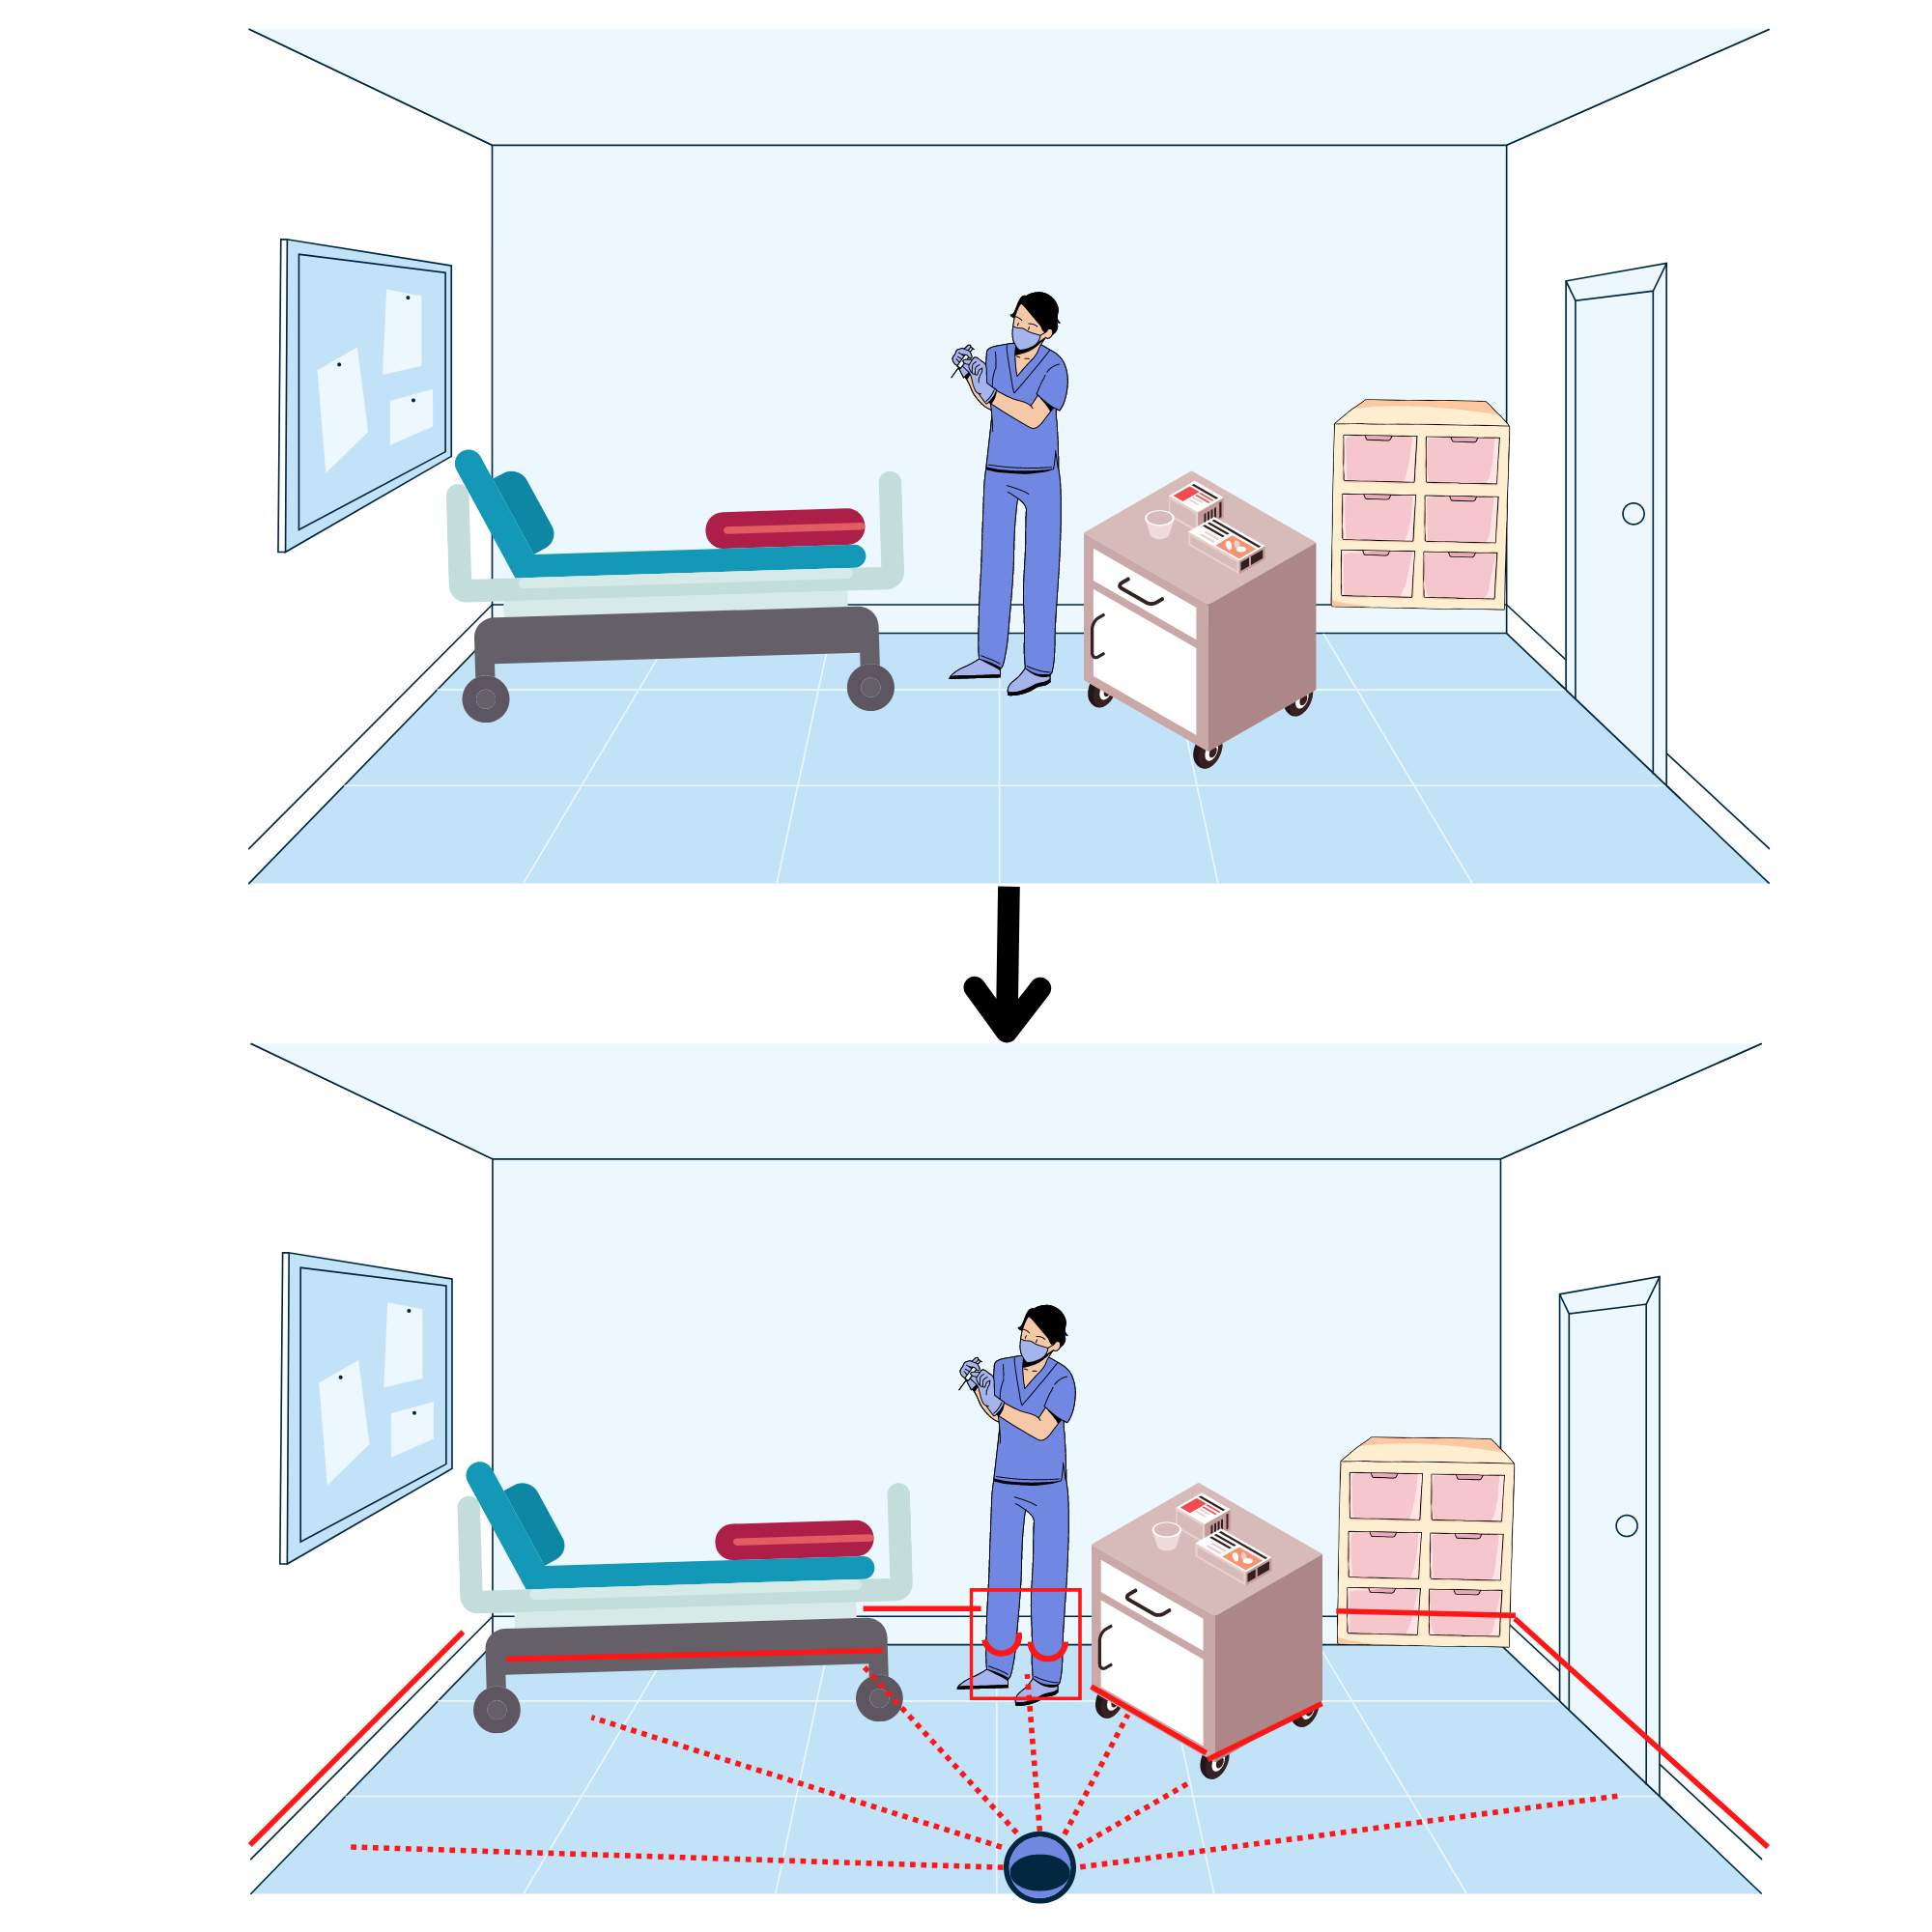
\includegraphics[scale=0.4]{bab4/ilustrasi_L.png}
    \caption{Ilustrasi Kerja Sistem Deteksi.} 
    % source : https://www.canva.com/design/DAFNOD4NtO8/fk5zN3JJ6QSwVgpEgwJ3jg/edit
    \label{fig:Ch04_ilustrasi}
\end{figure}

Pendeteksian dua jenis bentuk yaitu garis dan lingkaran cukup untuk dapat mewakili bentuk-bentuk umum yang biasanya ada di dalam ruangan. Bentuk garis merupakan bentuk umum yang dimiliki berbagai objek di dalam ruangan rumah sakit seperti dinding, meja, tempat tidur, dan sebagainya. Objek-objek dalam ruang yang memiliki bentuk lingkaran cukup terbatas jenisnya. Bentuk lingkaran yang memiliki ukuran seperti manusia juga biasanya jarang ditemukan di lingkungan rumah sakit. Manusia dapat dibedakan dengan objek lingkaran lainnya dengan menambahkan beberapa syarat yang sesuai dengan kriteria kaki manusia.

Sistem deteksi ini secara keseluruhan memiliki empat tahap pembuatan komponen sebelum disimulasikan secara utuh. Tahap-tahap tersebut ditunjukkan pada Gambar \ref{fig:Ch04_sistem_umum}.

    \begin{figure}[H]
        \centering
        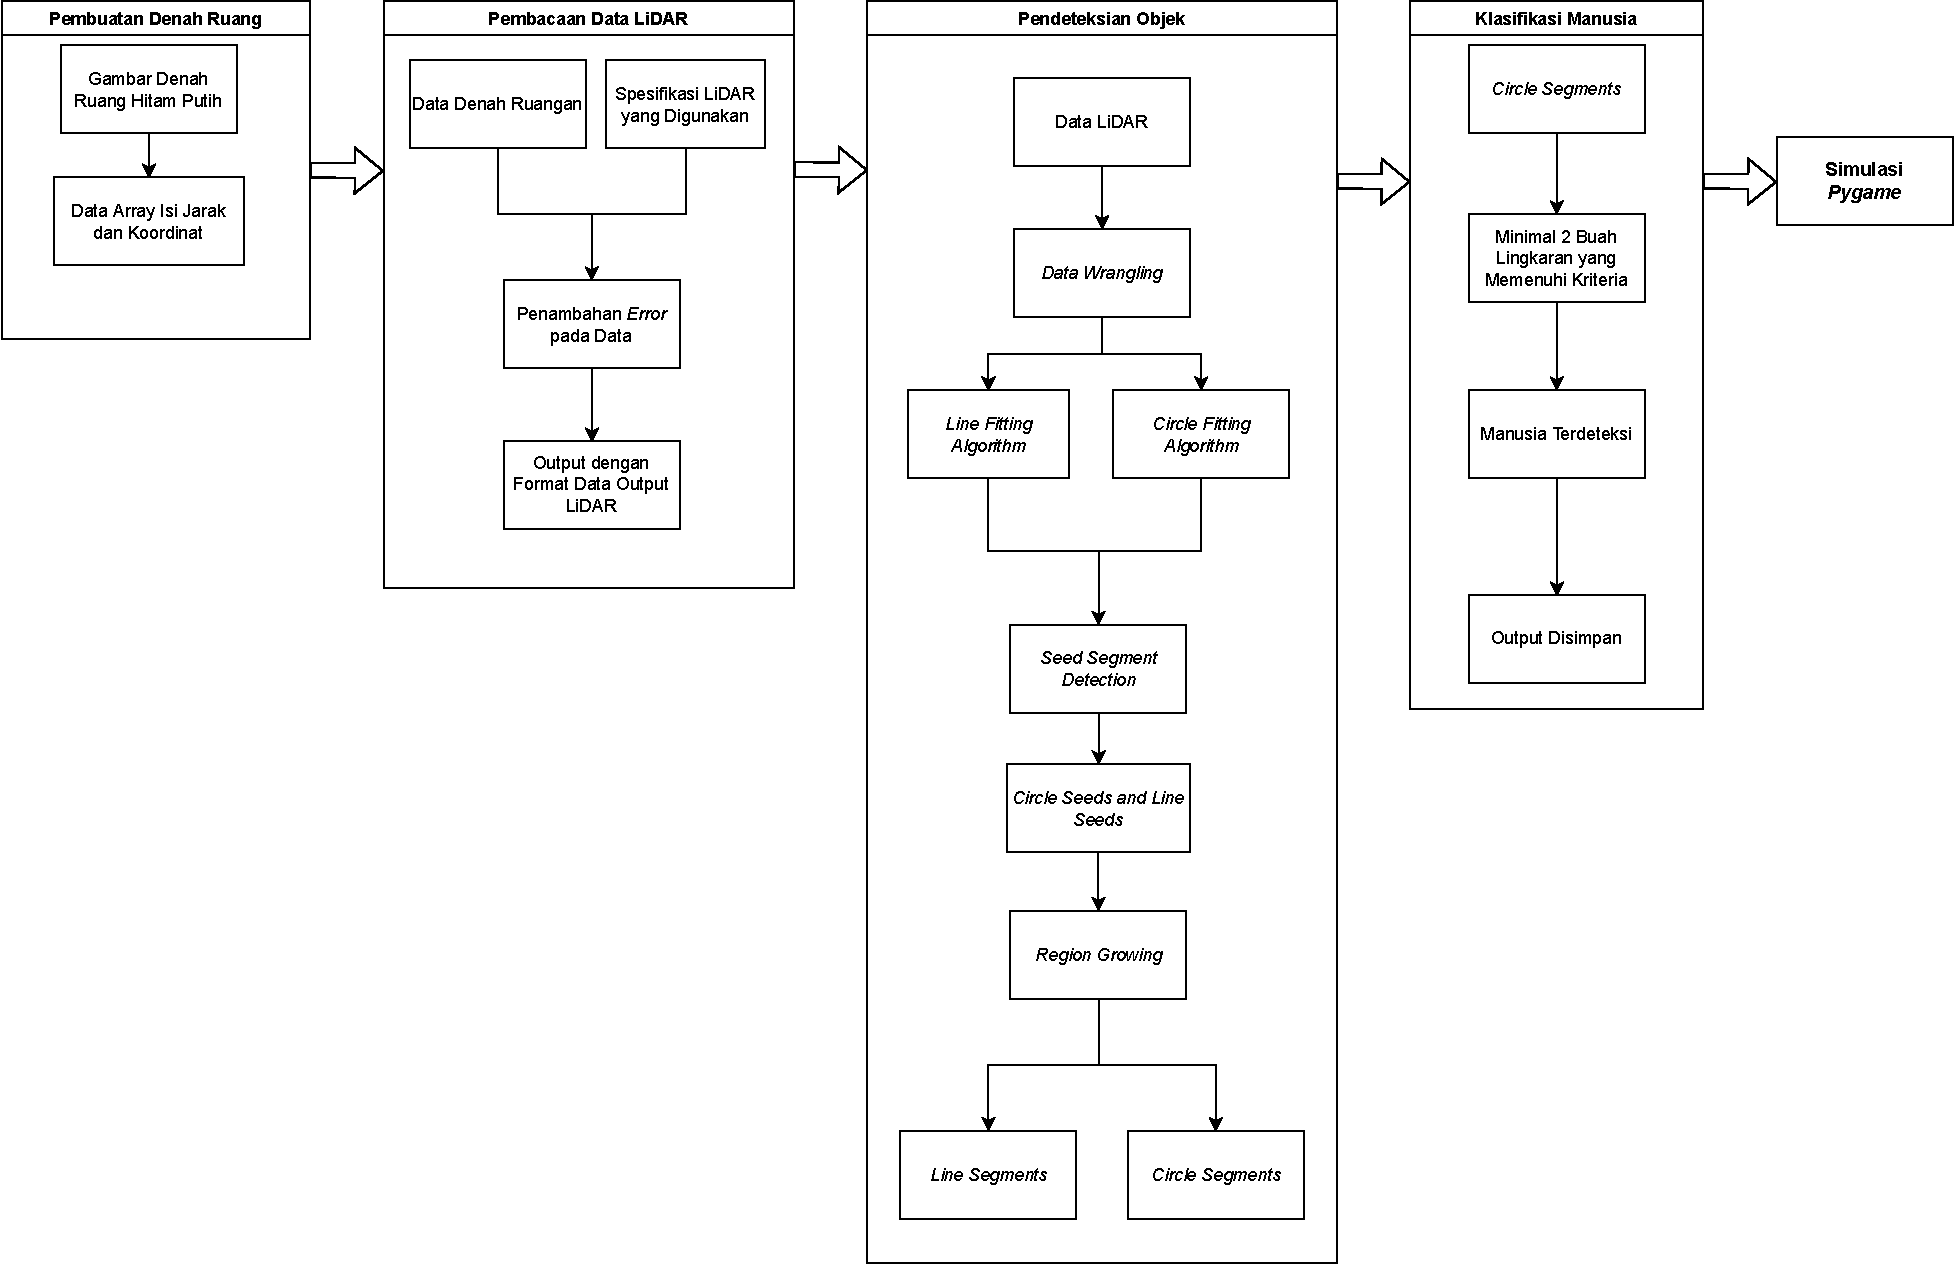
\includegraphics[width=\textwidth]{bab4/workflow_umum.pdf}
        \caption{Diagram Kerja Sistem secara Umum.}
        \label{fig:Ch04_sistem_umum}
    \end{figure}

Tahap pertama adalah pembuatan lingkungan yang akan digunakan. Masukkan data lingkungan untuk simulasi diperoleh dari gambar denah ruangan yang berwarna hitam putih. Gambar kemudian diubah menjadi data \textit{array} agar dapat dengan mudah diproses. Tahap selanjutnya adalah membuat program yang memberi luaran seperti luaran data mentah \lidar. Terdapat dua masukkan yang dibutuhkan untuk membuat program pada tahap ini yaitu data denah ruangan dan spesifikasi \lidar\ yang ingin digunakan. Spesifikasi \lidar\ digunakan sebagai penentu agar data yang dihasilkan dapat memiliki sifat semirip mungkin dengan bacaan \lidar\ asli. Data kemudian ditambah \textit{error} kemudian disusun sesuai format luaran data \lidar. Tahap selanjutnya adalah pendeteksian garis dan lingkaran. Data mentah \lidar\ perlu disusun menjadi format yang mudah diproses. Data-data tersebut akan dimasukkan ke dalam program pendeteksi garis dan lingkaran untuk kemudian dicari apakah ada sekelompok data yang memenuhi kriteria untuk dianggap sebagai \textit{seed}. \textit{Seed} kemudian dikembangkan menjadi garis atau lingkaran, segmen-segmen garis dan lingkaran disimpan untuk diproses pada tahap selanjutnya. Segmen-segmen garis nanti akan ditampilkan pada simulasi sementara segmen-segmen lingkaran akan dikelompokkan terlebih dahulu mana yang memenuhi kriteria untuk dianggap sebagai manusia kemudian ditampilkan pada simulasi. Penjelasan lebih lengkap mengenai diagram kerja dituliskan pada subbab \ref{sec:Persiapan}, subbab \ref{sec:Persiapan2}, subbab \ref{sec:Deteksi}, subbab \ref{sec:Fitting}, dan subbab \ref{sec:Klasifikasi}.

\subsection{Persiapan Denah Ruangan}
\label{sec:Persiapan}

Data proyek \textit{capstone} ini diperoleh tidak menggunakan sensor nyata yang digunakan dalam ruangan, data lingkungan dibuat dari gambar denah ruangan. Denah ruangan dibuat berdasarkan pengamatan dari lorong Gedung DTETI lantai 2. Area yang dijadikan landasan pembuatan denah ditunjukkan area berwarna pada Gambar \ref*{fig:Ch04_lantai_dteti}. 
\begin{figure}[H]
    \centering
    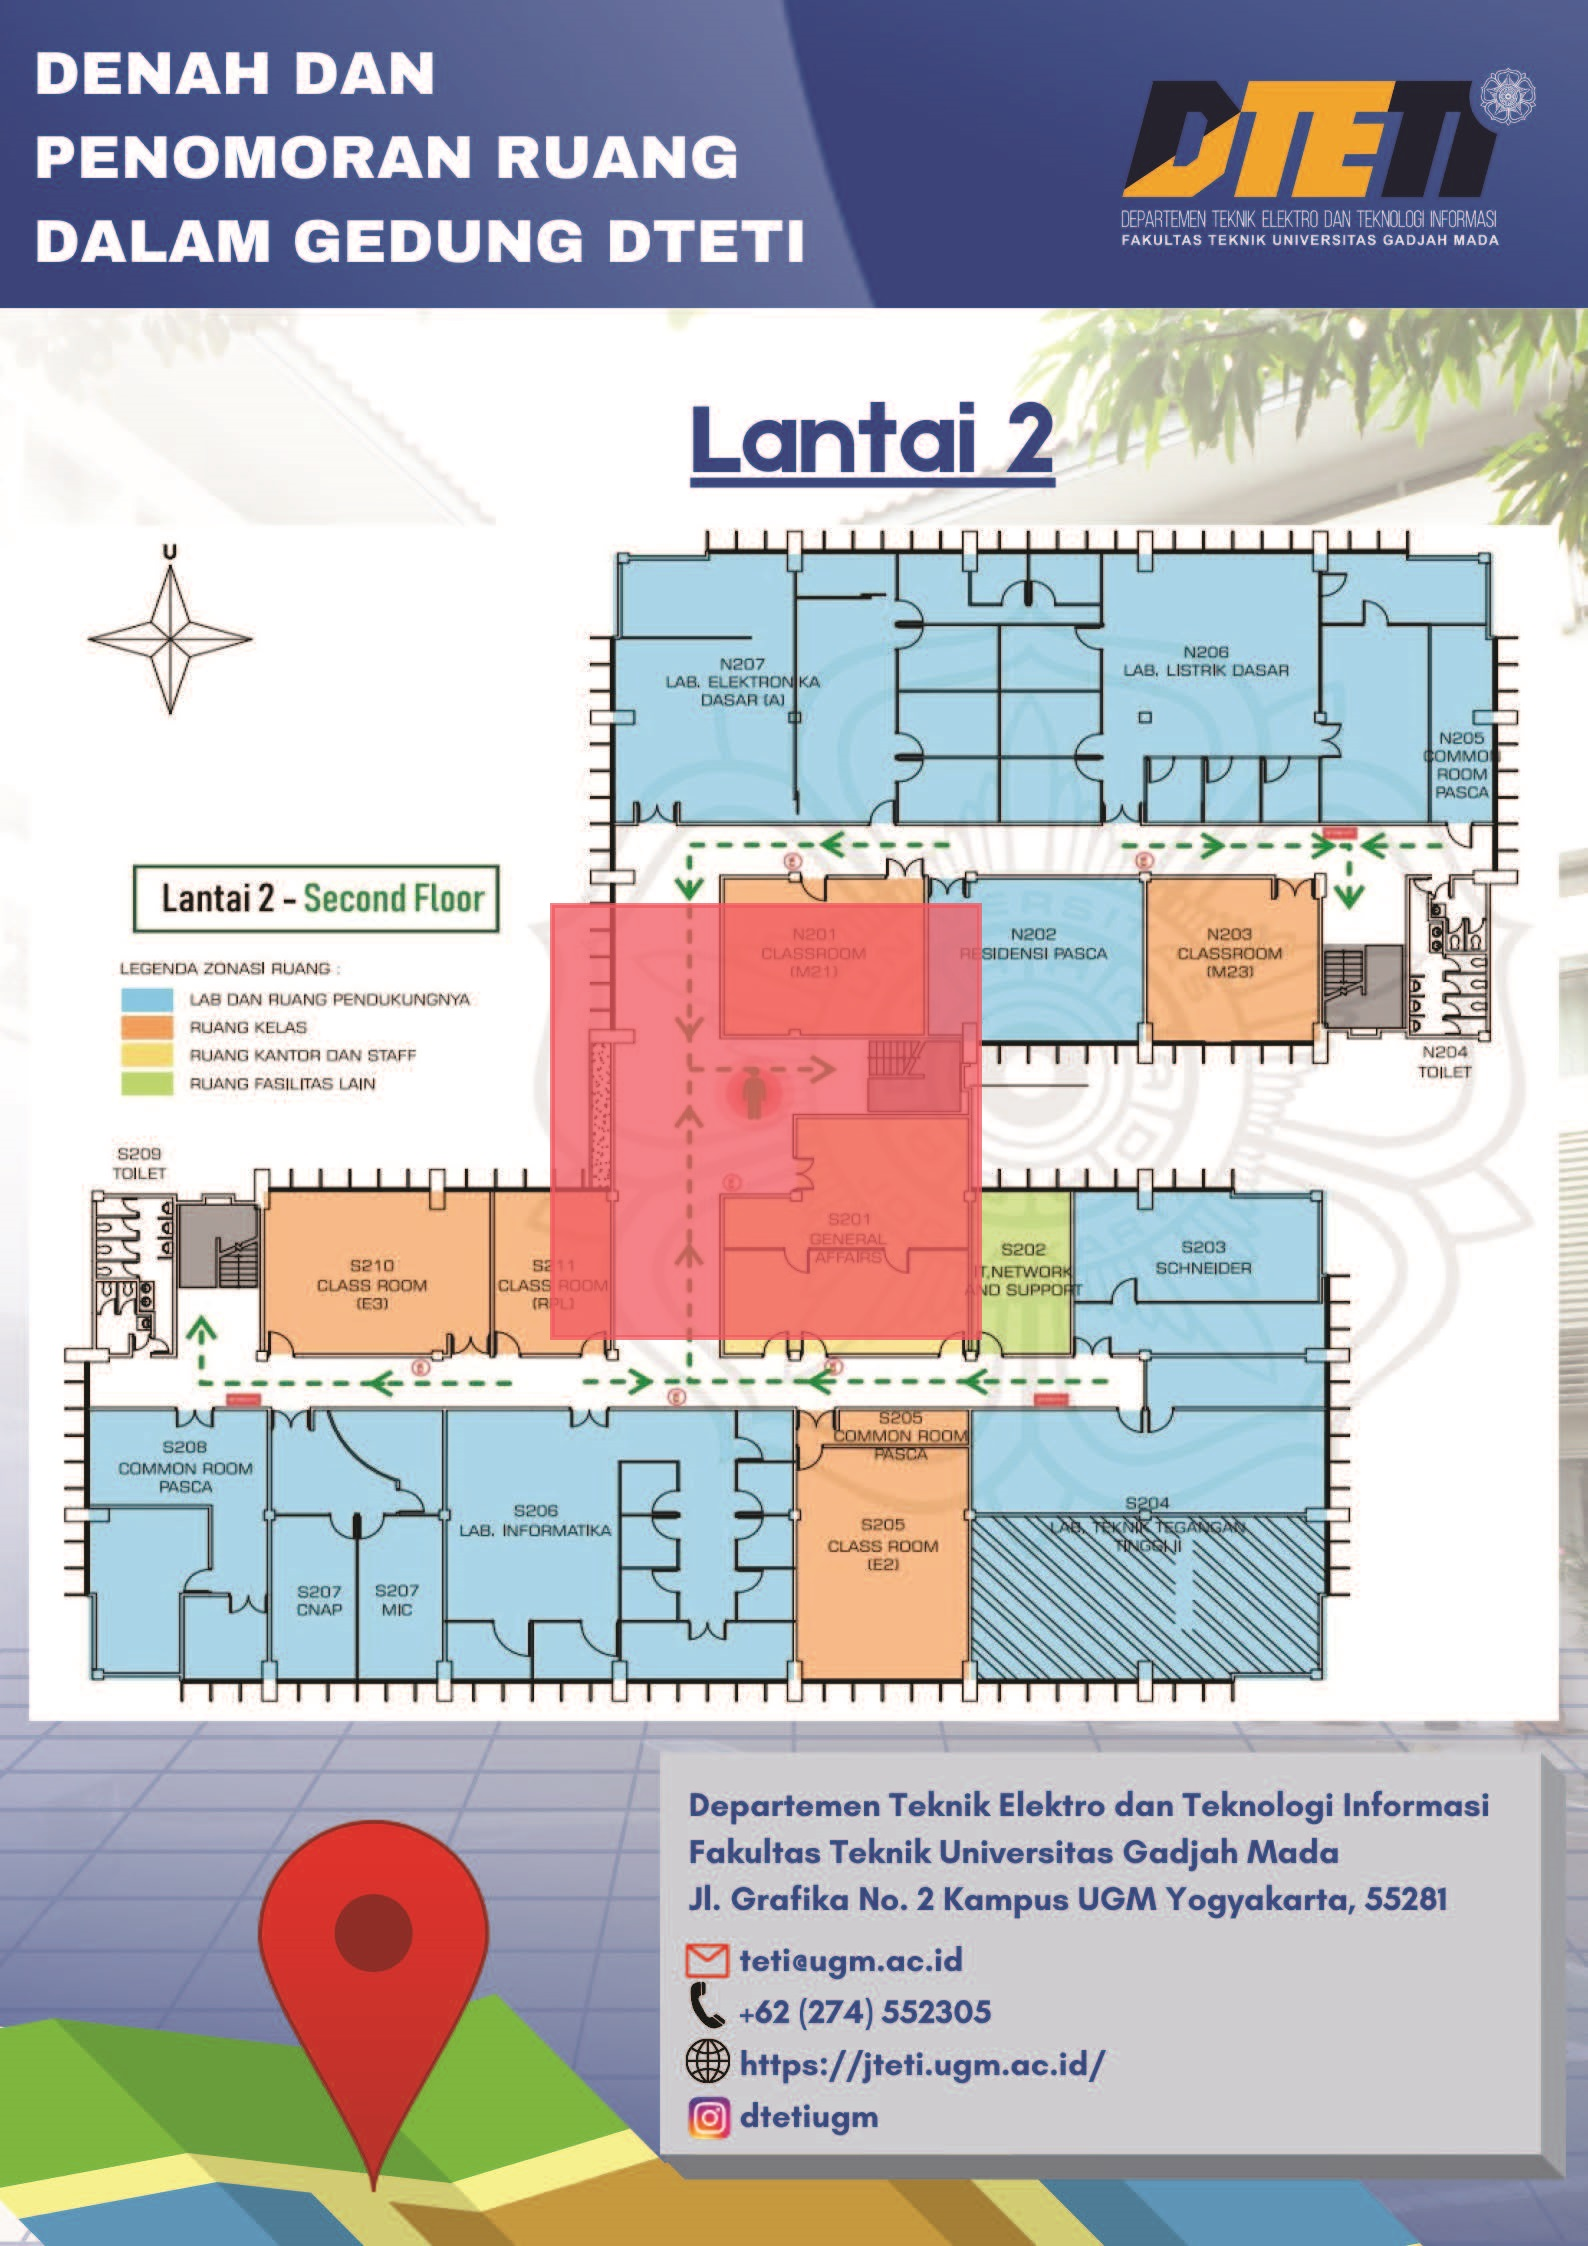
\includegraphics[width=0.7\textwidth]{bab4/denah-lantai-2-rev.jpg}
    \caption{Denah Lantai 2 Gedung DTETI UGM\cite{d00}.}
    \label{fig:Ch04_lantai_dteti}
\end{figure}

Denah ruangan dijadikan landasan ukuran pembuatan lorong yang akan dilalui robot pada simulasi. Denah diubah menjadi berwarna hitam putih dan ditambah beberapa objek berbentuk persegi empat dan lingkaran.
Terlihat pada Gambar \ref{Fig:Ch04_map1}, gambar denah hanya terdiri dari dua warna yaitu hitam dan putih. Warna putih mewakili ruang kosong sementara warna hitam mewakili objek nyata yang menerima pancaran sinar \lidar.

\begin{figure}[H]
    \centering
    \begin{subfigure}[b]{\textwidth}\centering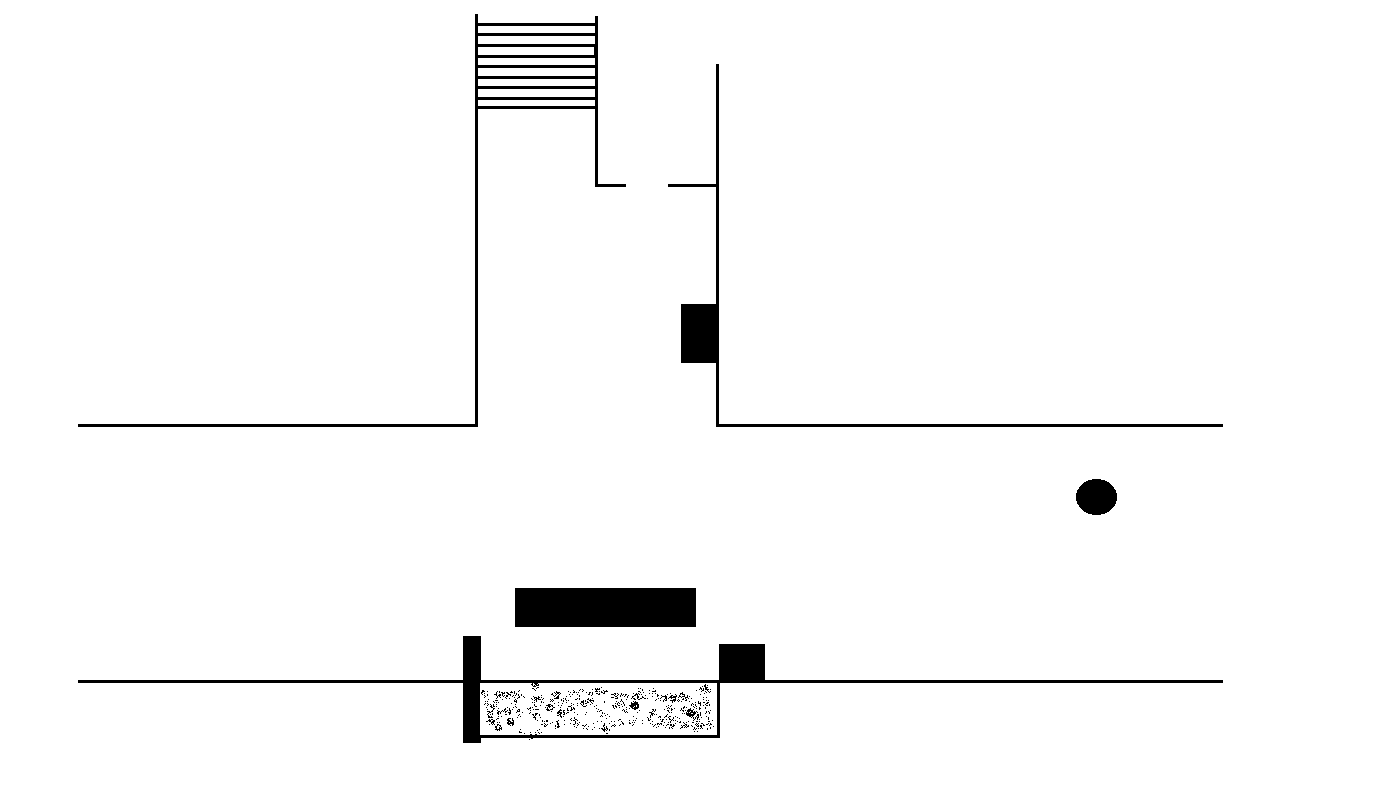
\includegraphics[scale=0.54]{bab4/map_dteti.png}\caption{Denah Ruangan.}\label{Fig:Ch04_map1}\end{subfigure}\\
    \begin{subfigure}[b]{\textwidth}\centering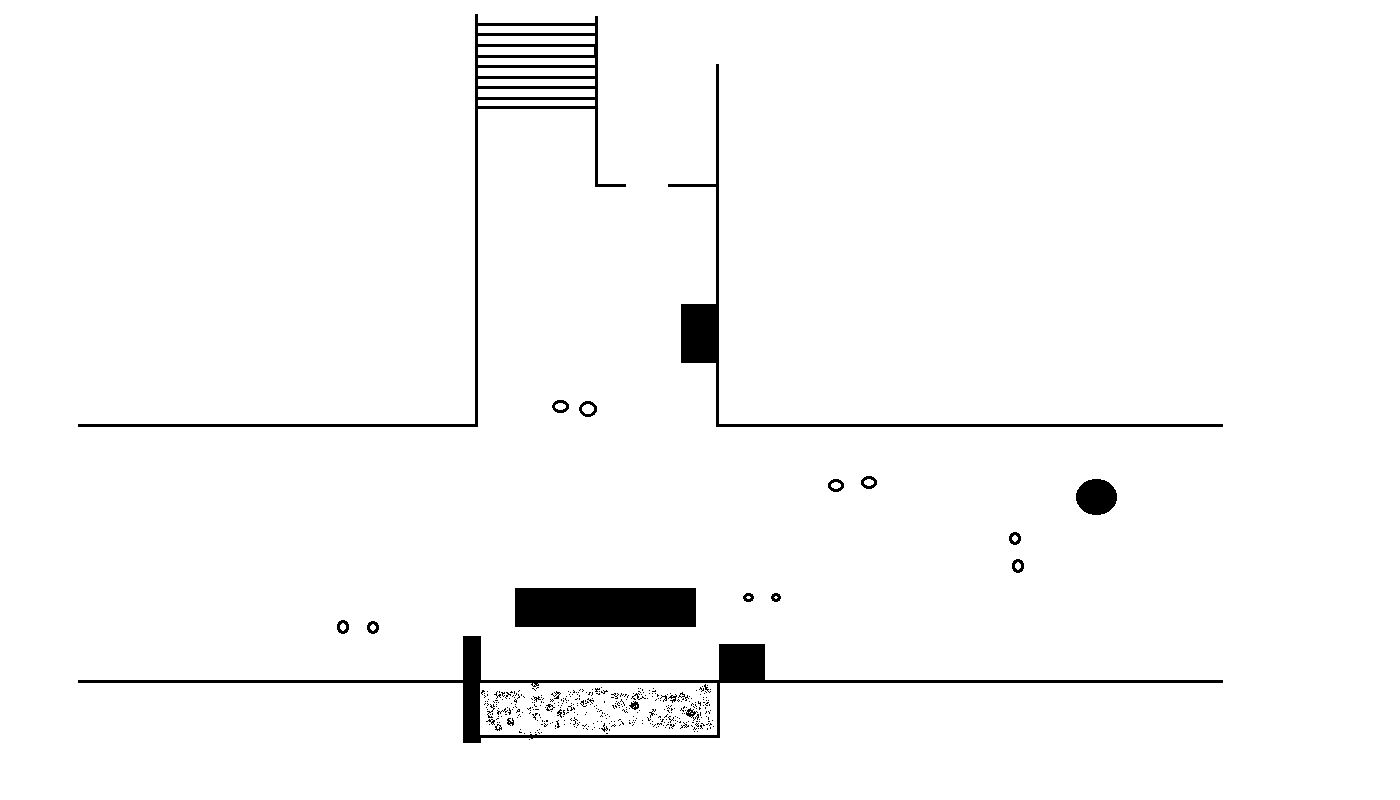
\includegraphics[scale=0.54]{bab4/map_dteti2.png}\caption{Denah Ruangan dengan Manusia.}\label{Fig:Ch04_map2}\end{subfigure}
    \caption{Pembuatan Denah Ruangan}
    \label{fig:Ch04_denahruang}
\end{figure}

Pada Gambar \ref{Fig:Ch04_map2}, manusia ditunjukkan dengan gambar dua buah lingkaran yang berdekatan. Denah awal berisi denah ruangan yang akan dilalui robot, kemudian gambar kedua adalah denah yang sudah ditambahi kaki manusia yang berbentuk sepasang objek lingkaran. Lingkaran-lingkaran ini memiliki jari-jari yang berukuran antara 4,5 cm hingga 8,5 cm. Gambar diproses menjadi data jarak dan posisi objek dengan 1 pixel gambar menggambarkan 1 cm jarak asli.

\begin{figure}[H]
    \centering
    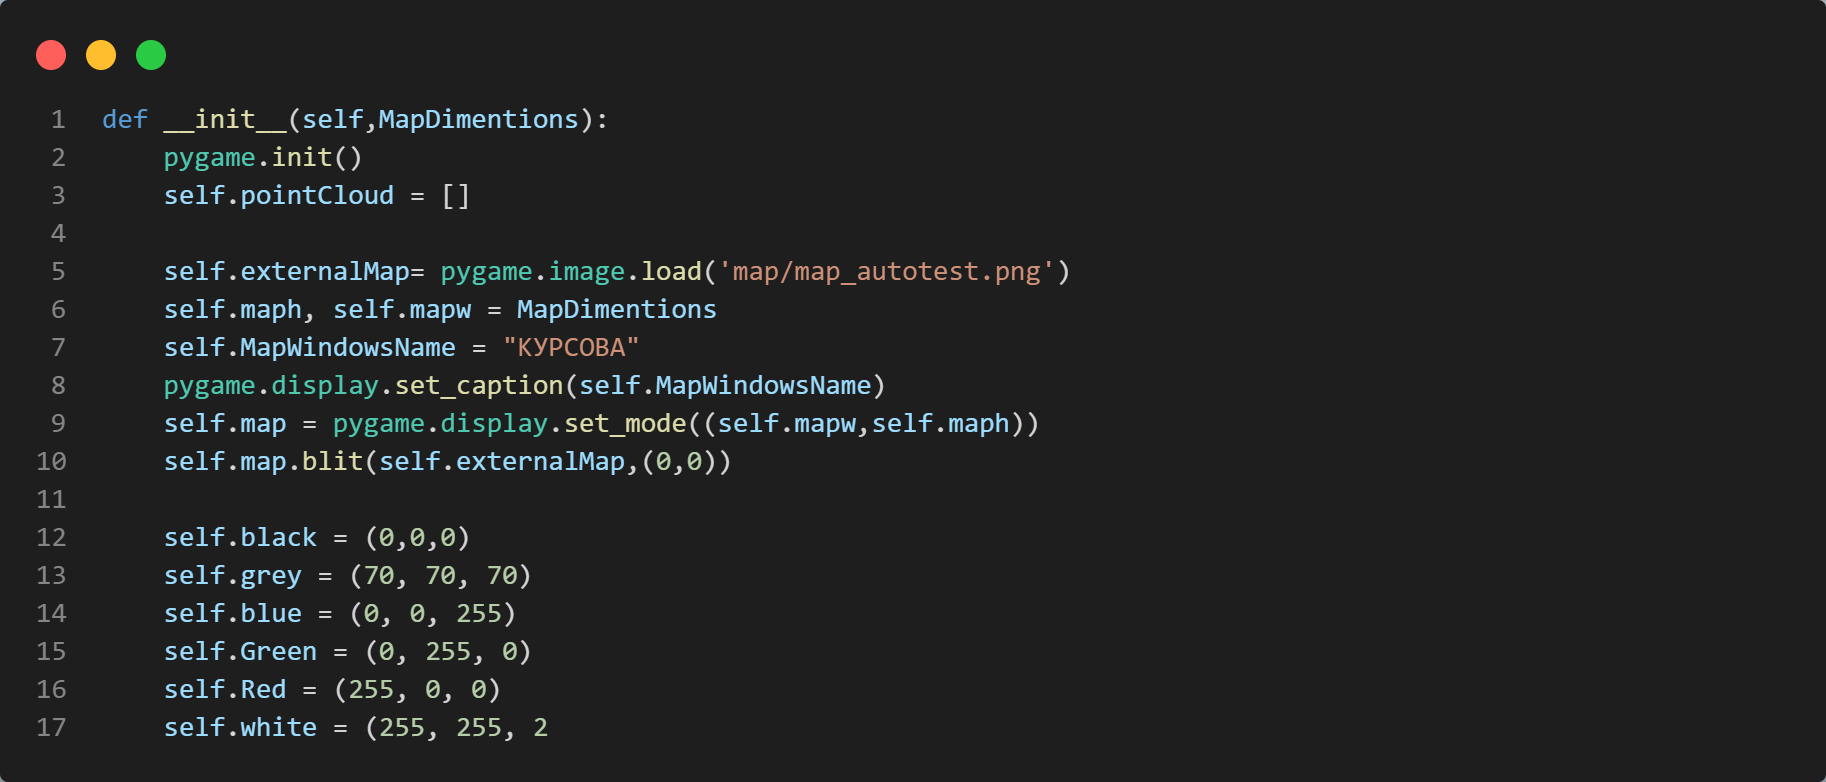
\includegraphics[width=\textwidth]{snippet/build_map.png}
    \caption{Potongan Program Pembacaan Gambar Denah.}
    \label{fig:Ch04_program_denah}
\end{figure}

Potongan program untuk membaca denah yang berupa gambar terlihat pada Gambar \ref{fig:Ch04_program_denah}. Langkah pertama adalah dengan memasukkan gambar png denah ke dalam variabel \textit{self.externalMap} melalui \textit{pygame}. Langkah selanjutnya adalah mengatur ukuran denah dan mengatur nama denah baru yang akan ditampilkan pada layar. Langkah terakhir adalah menggambar data yang diterima dari gambar denah ke tampilan denah yang baru dibuat. Variabel-variabel warna dibuat sebagai persiapan jika nantinya ingin menampilkan warna-warna tersebut dalam denah.
\begin{figure}[H]
    \centering
    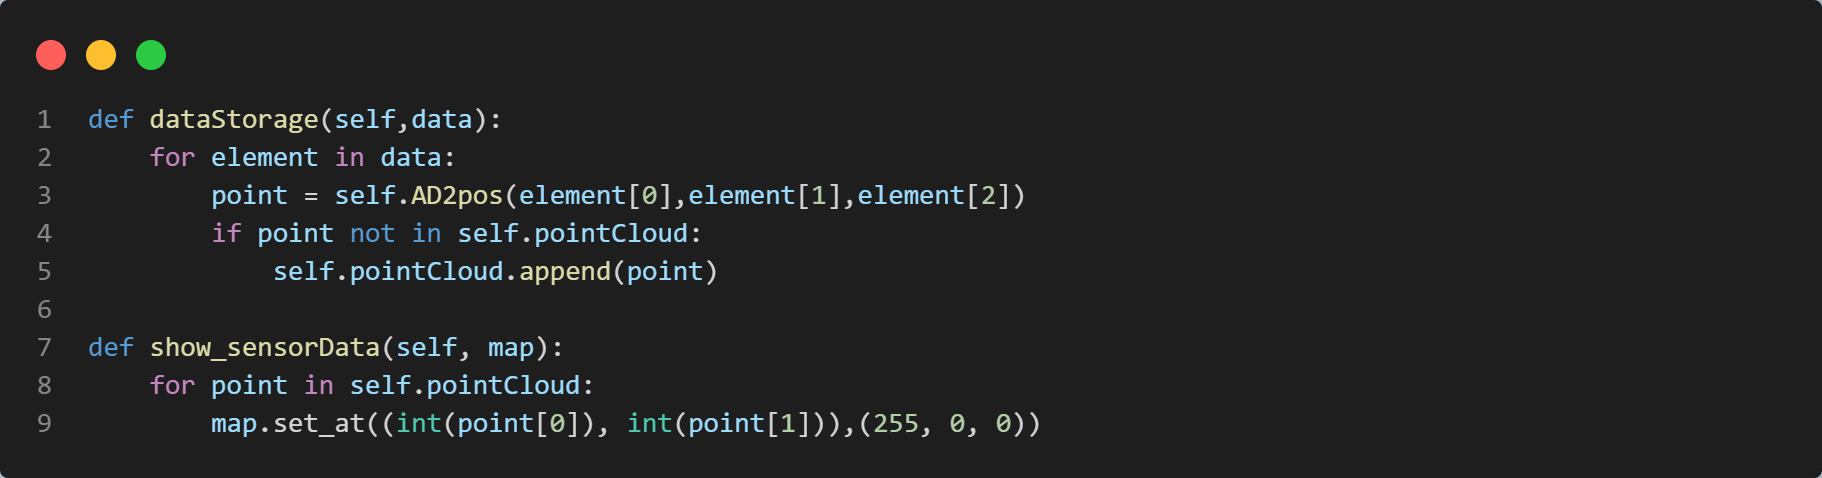
\includegraphics[width=\textwidth]{snippet/build_map2.png}
    \caption{Potongan Program Penyimpanan Data Denah.}
    \label{fig:Ch04_program_denah2}
\end{figure}

Gambar \ref{fig:Ch04_program_denah2} menunjukkan potongan program untuk menyimpan data sebelum ditampilkan pada simulasi. Fungsi \textit{dataStorage} adalah untuk menyimpan hasil bacaan sensor sehingga data pemindaian \lidar\ dari waktu ke waktu tidak akan hilang. Gambar utuh denah ruangan dapat ditampilkan jika fungsi tersebut diaktifkan. Fungsi \textit{show\_sensorData} adalah fungsi yang berguna untuk menampilkan titik-titik yang tersimpan pada fungsi sebelumnya. Titik-titik ini ditampilkan pada simulasi \textit{pygame} dengan warna merah yang diwakilkan pada program dengan kode warna $(255,0,0)$. 


\subsection{Persiapan Data \lidar}
\label{sec:Persiapan2}

Robot akan membaca data lingkungan sesuai spesifikasi \lidar\ yang digunakan. Data objek yang terdeteksi \lidar\ akan dibuat menjadi data yang berisi jarak dan sudut dari objek terdeteksi. Satu putaran \lidar\ memiliki jumlah data yang berbeda-beda sesuai spesifikasi \lidar\ yang digunakan. Jumlah data bacaan \lidar\ yang memiliki jangkauan sudut $360 \degree$ dapat dihitung dengan persamaan \ref*{eqn:SIR1}.
    \begin{align}
        \label{eqn:SIR1}
        Sample\ Rate\ (SR) = \frac{sample\ frequency}{motor\ speed}
    \end{align}
dengan \textit{sample rate} merupakan jumlah data yang diterima dalam satu putaran, \textit{sample frequency} menunjukkan frekuensi kecepatan pembacaan \lidar, dan \textit{motor speed} adalah kecepatan motor dalam \lidar\ untuk memutar laser. 

Nilai jarak dan sudut yang diperoleh \lidar\ akan selalu memiliki nilai ketidakpastian \textit{(uncertainty)}. Nilai ini merupakan perbedaan antara jarak yang diterima \lidar\ dengan jarak asli objek, perbedaan ini dapat diakibatkan oleh berbagai hal seperti kondisi permukaan objek, kualitas manufaktur \lidar, sudut tembakan laser \lidar, dan posisi peletakan \lidar\cite{d0}. Proyek sistem deteksi ini hanya akan memperhitungkan \textit{error} yang dicantumkan pada spesifikasi \lidar. %https://doi.org/10.5194/wes-7-413-2022 
Data yang diperoleh dari objek diam yang dipindai \lidar\ juga dapat memberikan hasil bacaan posisi sudut berbeda dalam setiap pemindaian. Hal ini disebabkan oleh frekuensi penembakkan sinar \lidar\ yang berbeda dengan kecepatan motor yang memutar \lidar\ 2D.

\subsection{Deteksi Segmen Garis dan Lingkaran}
\label{sec:Deteksi}

Ruangan yang telah dibaca oleh \lidar\ hanya akan menghasilkan data mentah yang berisi jarak dan posisi objek yang perlu diproses lebih lanjut agar dapat berguna agar mendukung fungsi-fungsi robot lainnya untuk mengidentifikasi lingkungan. Data yang diperoleh berupa data dua dimensi sehingga objek-objek di sekitar robot hanya dapat dikelompokkan menjadi bentuk-bentuk dua dimensi. 

\begin{figure}[H]
    \centering
    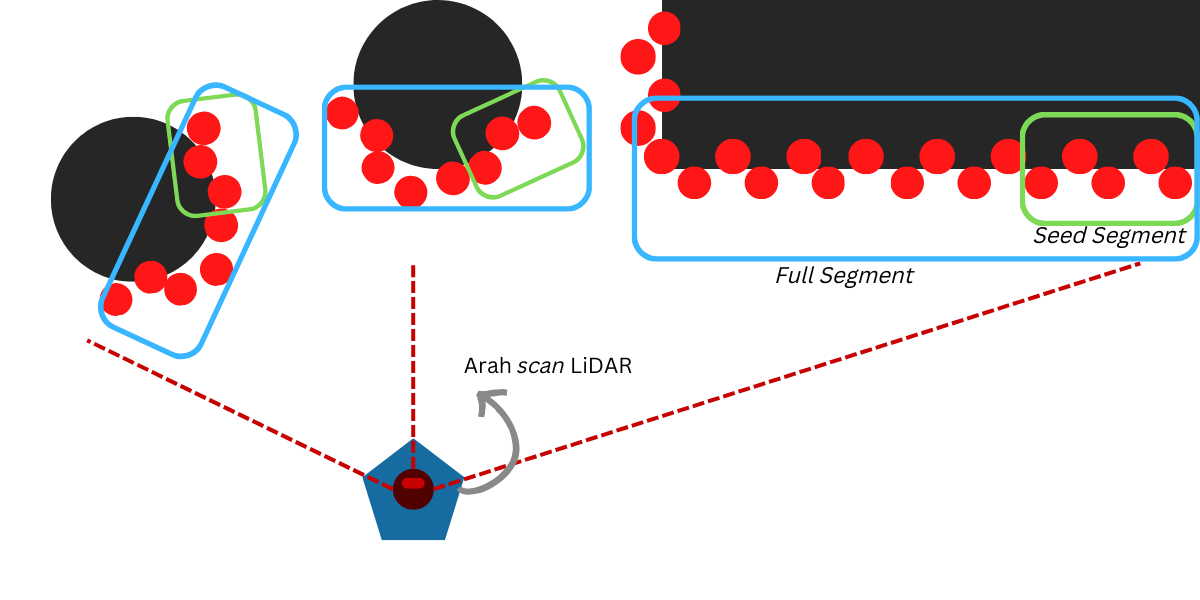
\includegraphics[scale=0.35]{bab4/algoritma.png}
    \caption{Ilustrasi \textit{Seed-growing Algorithm} pada \lidar.}
    \label{fig:Ch04_ilustrasi_algoritma}
\end{figure}

Banyak jenis variasi algoritma yang dapat digunakan untuk mengidentifikasi data 2D \lidar. Proyek \textit{capstone} ini akan menggunakan metode \textit{seed-growing algorithm}\cite{d3}.  
% this paper which uses a variation of the famous split and merge algorithm in order to process 2d lidar data producing a set of line segments that can be used in slam applications this paper claims that this variation can perform better than the original split and merge algorithm in terms of efficiency correctness and precision.\newline 
% BASA BASI:
% Using pure laser scan data to detect human legs can be a 
% complicated problem. Some researchers utilize both vision 
% sensors and laser range scanners [3].
% [3] Kim,  Chung, Detection and tracking of human legs for a mobile service robot[P]. Advanced Intelligent 
% Mechatronics (AIM), 2010 IEEE/ASME International Conference 
% on,2010.
% . Another type of method is to abandon 
% the laser sensor and directly use RGBD-based deep attention 
% models to detect and locate people [4]. This method is more 
% accurate and correspondingly consumes more computing 
% resources than ordinary vision solutions.
% The goal of our work is to build a system that can detect 
% human legs around the robot based on pure laser scan data and 
% minimize false positives. Our leg detection system references 
% the random forest model mentioned above and includes a series 
% of mechanisms like feature filter and map mask to detect human 
% legs without computer vision
% As we can see in Fig 1, our system requires the robot to build
% a two-dimensional map of the surrounding scene using lidar first.
% Then, the robot uses the laser scan data and the already built map 
% to locate itself and update the surrounding environment data in 
% real time.
% The pre-processing process is the process of building a map
% for the environment using the SLAM methods based on the laser 
% scan data.
Algoritma ini secara umum terbagi menjadi dua tahap yaitu \textit{seed-segment detection} dan \textit{region growing} yang dapat dilihat pada Gambar \ref*{fig:Ch04_ilustrasi_algoritma}. \textit{Seed-segment detection} bertujuan untuk mencari kelompok data yang akan digunakan untuk mencari data lain kemudian dimasukkan ke dalam kelompoknya. Setelah kelompok \textit{seed} ditemukan maka selanjutnya dilakukan \textit{region growing}. \textit{Region growing} digunakan untuk mencari titik-titik di sekitar \textit{seed} untuk ditambahkan hingga menjadi segmen garis atau lingkaran yang utuh. Cara kerja kedua tahap tersebut terus diulang-ulang dalam satu kali pembacaan data \lidar\ hingga semua data yang terbaca dapat teridentifikasi. Cara kerja \textit{seed-segment detection} dapat dilihat pada algoritma \ref{algo:algo1} dan cara kerja \textit{region growing} dapat dilihat pada algoritma \ref{algo:algo2}.

\begin{algorithm}[H]
    \caption{Seed-segment Detection} 
    \label{algo:algo1}
    \glsadd{N_p}
    \begin{algorithmic}[1]
        \Require $\textbf{N}_{p}\glsadd{N_p},\epsilon\glsadd{epsilon}, \glsadd{delta}\delta, \glsadd{Snum}S_{num}, \glsadd{Pmin}P_{min}$  
        \State Initialization flag = true
        \For {$i=1 \to (\textbf{N}_{p}\glsadd{N_p}-\textbf{P}_{min})$}
            \State $j \gets i + \textbf{S}_{num}$
            \State fit \glsadd{segmen}\textbf{Seed}$(i,j)$
            \For {$k=i \to j$}
                \State obtain the predicted point or the next point $P'_{k}$
                \State $d_{1} \gets distance\ from\ P_{k}\ to\ P'_{k}$
                \If{$d_{1}>\glsadd{delta}\delta$}
                    \State $flag=false$
                    \State break
                \EndIf
                \State $d_{2}\gets distance\ from\ P_{k}\ to\ \glsadd{segmen}\textbf{Seed} (i,j)$
                \If{$d_{2}>\epsilon\glsadd{epsilon}$}
                    \State $flag = false$
                    \State break
                \EndIf 
            \EndFor
            \If{$flag==true$}
                \State return $\glsadd{segmen}\textbf{Seed} (i,j)$
            \EndIf
        \EndFor
    \end{algorithmic} 
\end{algorithm}

Pada algoritma \ref*{algo:algo1}, $N_p$ merupakan jumlah titik yang terdeteksi. $\glsadd{Snum}S_{num}$ merupakan jumlah titik yang diperlukan untuk \textit{seed-segment} dan $\glsadd{Pmin}P_{min}$ jumlah titik minimal yang dibutuhkan untuk membuat segmen. Segmen garis dari titik $i$ menuju titik $j$ diwakilkan dengan $Seed(i,j)$, sementara nilai $\epsilon\glsadd{epsilon}$ adalah jarak terdekat garis dan $\glsadd{delta}\delta$ adalah jarak antar titik seperti yang dijelaskan pada Gambar \ref{fig:Ch04_epsdelta}.

\begin{figure}[H]
    \centering
    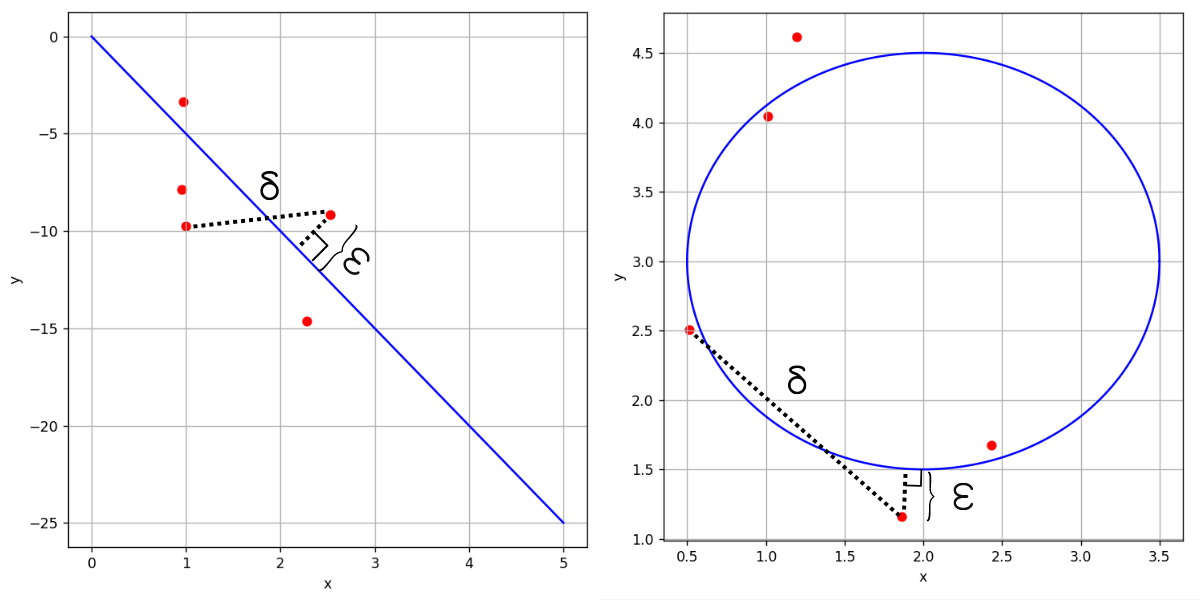
\includegraphics[scale=0.45]{bab4/eps_delta.png}
    \caption{Jarak $\epsilon$ dan $\delta$ pada Garis dan Titik.}
    \label{fig:Ch04_epsdelta}
\end{figure}
Nilai $\epsilon\glsadd{epsilon}_{line}$ dan $\epsilon\glsadd{epsilon}_{circle}$ dapat dihitung menggunakan persamaan jarak titik ke garis dan titik ke lingkaran yang ditampilkan pada Tabel \ref*{tab:Persamaan_Matematis}. Nilai $\glsadd{delta}\delta_{line}$ dan $\glsadd{delta}\delta_{circle}$ dapat juga dilihat pada tabel tersebut yaitu menggunakan rumus jarak titik ke titik. Berbagai persamaan matematika lainnya juga digunakan untuk menyusun sistem deteksi ini. Fungsi dan tujuan persamaan-persamaan tersebut ditampilkan dan dijelaskan pada Tabel \ref*{tab:Persamaan_Matematis}.

\begin{longtable}{|c|L{2cm}|L{4cm}|L{5.5cm}|}
    \caption{Persamaan Matematis dalam \textit{Features Detection}}
    \label{tab:Persamaan_Matematis}
    \vspace{-0.75em}\\
    \hline
   \multicolumn{1}{|c|}{\textbf{No.}} 
   & \multicolumn{1}{|c|}{\textbf{Nama Fungsi}} 
   & \multicolumn{1}{|c|}{\textbf{Fungsi}} 
   & \multicolumn{1}{|c|}{\textbf{Deskripsi}}\\ \hline
    {1.}
      & {Persamaan Garis dengan Gradien} 
      & \multicolumn{1}{|c|}{$y=mx+b$}
      & Persamaan garis lurus dengan $m$ sebagai gradien dan $b$ sebagai titik potong sumbu $y$.
      \\ \hline
    {2.}
    & {Persamaan Garis Umum} 
    & \multicolumn{1}{|c|}{$Ax+By+C=0$}
    & Persamaan garis dalam bentuk umum di bidang sumbu $x$ dan $y$.
    \\ \hline
    {3.}
    & {Persamaan Garis dari Dua Titik} 
    & \multicolumn{1}{|c|}{\large$\frac{y-y_1}{y_2-y_1}=\frac{x-x_1}{x_2-x_1}$}
    & Persamaan garis yang dapat diperoleh jika diketahui dua titik $(x_1,y_1)$ dan $(x_2,y_2)$. 
    \\ \hline
    {4.}
    & {Jarak Titik ke Titik} 
    & \multicolumn{1}{|c|}{$\sqrt{(x_2-x_1)^2+(y_2-y_1)^2}$}
    & Persamaan untuk menghitung jarak antar dua titik yaitu titik $(x_1,y_1)$ dan $(x_2,y_2)$.
    \\ \hline
    {5.}
    & {Jarak Titik ke Garis}
    & \multicolumn{1}{|c|}{\large$\frac{|Ax_i+By_i+C|}{\sqrt{A^2+B^2}}$}
    & Persamaan untuk menghitung jarak dari sebuah titik $(x_i,y_i)$ menuju sebuah garis dengan persamaan $Ax+By+C=0$.
    \\ \hline
    {6.}
    & {Jarak Titik ke Lingkaran}
    & \multicolumn{1}{|c|}{$\sqrt{|(x_i-x_c\glsadd{x_c})^2+(y_i-y_c\glsadd{y_c})^2|}-r_c\glsadd{r_c}$}
    & Persamaan untuk menghitung jarak dari sebuah titik $(x_i,y_i)$ menuju sebuah lingkaran dengan persamaan $(x-x_c)^2+(y-y_c)^2+R^2=0$.
    \\ \hline
    {7.}
    & {Jarak Titik ke Titik dalam Busur Lingkaran}
    & \multicolumn{1}{|c|}{
        \begin{tabular}{c}
            \small $\theta\glsadd{theta}=\arctan \left(\frac{\mfrac{y_c\glsadd{y_c}-y_2}{x_c\glsadd{x_c}-x_2} - \mfrac{y_c\glsadd{y_c}-y_1}{x_c\glsadd{x_c}-x_1}}{1+\left(\mfrac{y_c\glsadd{y_c}-y_2}{x_c\glsadd{x_c}-x_2}\right) \left(\mfrac{y_c\glsadd{y_c}-y_1}{x_c\glsadd{x_c}-x_1}\right)}\right)$\\ \\
            $jarak = \left(\frac{\theta\glsadd{theta}}{360\degree}\right)\times 2\pi r_c\glsadd{r_c}$
        \end{tabular}}
    & Persamaan untuk menghitung jarak busur lingkaran dengan pusat $(x_c\glsadd{x_c},y_c\glsadd{y_c})$ dan jari-jari $r_c\glsadd{r_c}$. Sebuah busur tersebut memiliki dua titik di ujung yaitu titik $(x_1,y_1)$ dan titik lain $(x_2,y_2)$.
    \\ \hline

    {8.}
    & {Titik Potong Dua Garis}
    & \multicolumn{1}{|c|}{$
        \begin{pmatrix}
          -m_1 & 1\\
          -m_2 & 1
        \end{pmatrix}
        \begin{pmatrix}
            x_k\\
            y_k
          \end{pmatrix} =
        \begin{pmatrix}
            b_1\\
            b_2
          \end{pmatrix}
      $}
    & Titik perpotongan antara dua persamaan garis $y=m_1x+b_1$ dan $y=m_2x+b_2$ dapat digambarkan dengan persamaan matriks tersebut yang nantinya dapat menghasilkan titik perpotongan $(x_k,y_k)$.
    \\ \hline
    {9.}
    & {Proyeksi Titik ke Garis}
    & \multicolumn{1}{|c|}{
        \begin{tabular}{c}
        $m_2=-\frac{1}{m}$\\ \\
        $y = m_2x+c_2$\\ \\
        $x_{k} = -\frac{(b-c_2)}{(m-m2)}$\\ \\
        $y_{k} = m_2x_{k}+c_2$
        \end{tabular} }
    & Fungsi untuk menghitung titik proyeksi $(x_k,y_k)$ dari sebuah titik $(x,y)$ di luar sebuah garis $y=mx+b$ sehingga apabila ditarik garis dari titik $(x,y)$ menuju $(x_k,y_k)$ maka garis tersebut akan tegak lurus dengan garis $y=mx+b$.
    \\ \hline

    {10.}
    & {Proyeksi Titik ke Lingkaran}
    & \multicolumn{1}{|c|}{
        \begin{tabular}{c}
        $\theta\glsadd{theta} = arctan \left( \frac{y_i-y_c\glsadd{y_c}}{x_i-x_c\glsadd{x_c}}\right)$\\ \\
        $x_{k} = x_c\glsadd{x_c} + r_c\glsadd{r_c} \cos \theta\glsadd{theta}$\\ \\
        $y_{k} = y_c\glsadd{y_c} + r_c\glsadd{r_c} \sin \theta\glsadd{theta}$
        \end{tabular} }
    & Fungsi untuk menghitung titik proyeksi $(x_k,y_k)$ dari sebuah titik $(x_i,y_i)$ di luar sebuah lingkaran $(x-x_c)^2+(y-y_c)^2+R^2=0$ sehingga apabila ditarik garis dari titik $(x,y)$ menuju $(x_k,y_k)$ maka jarak garis tersebut adalah jarak terdekat titik $(x_i,y_i)$ dengan lingkaran.
    \\ \hline

    {11.}
    & {Koordinat Polar dan Kartesius}
    & \multicolumn{1}{|c|}{
        \begin{tabular}{c}
            $x = r\ cos \theta\glsadd{theta}$\\ \\ 
            $y = r\ sin \theta\glsadd{theta}$
        \end{tabular}}
    & Fungsi untuk mengubah hasil bacaan \lidar\ yang berupa koordinat polar menjadi koordinat kartesius sehingga lebih mudah untuk diproses.
    \\ \hline
   \end{longtable}
Tabel \ref*{tab:Persamaan_Matematis} menjelaskan jenis-jenis persamaan yang digunakan dalam program. Persamaan-persamaan ini digunakan untuk membantu perhitungan dan memperoleh data dari kumpulan titik-titik yang dibaca \lidar. Persamaan-persamaan tersebut berfungsi dari proses pembacaan data \lidar\ hingga proses klasifikasi manusia.

\begin{algorithm}[H]
    \caption{Region Growing} 
    \label{algo:algo2}
    \begin{algorithmic}[1]
        \Require $\glsadd{segmen}\textbf{Seed} (i,j),\textbf{N}_{p}\glsadd{N_p}, \textbf{P}_{min}, \textbf{L}_{min}, \epsilon\glsadd{epsilon}$ 
        \State Initialization: $\textbf{Line}(P_{b},P_{f})\gets \glsadd{segmen}\textbf{Seed} (i,j),\textbf{L}_{l}=0, \textbf{P}_{l}=0 $
        \State $\textbf{P}_{f}=j+1, \textbf{P}_{b}=i-1$
        \While{$distance(\textbf{P}_{f}, \textbf{Line}<\epsilon\glsadd{epsilon})$}
            \If{$\textbf{P}_{f}>\textbf{N}_{p}\glsadd{N_p}$}
                \State break
            \Else
                \State refit $\textbf{Line}(\textbf{P}_{b}, \textbf{P}_{f})$
            \EndIf
            \State $P_{f} \gets P_{f}+1$
        \EndWhile
        \State $P_{f} \gets P_{f} -1 $
        \While{$distance(\textbf{P}_{b}, \textbf{Line}<\epsilon\glsadd{epsilon})$}
            \If{$\textbf{P}_{b}<1$}
                \State break
            \Else
                \State refit $\textbf{Line}(\textbf{P}_{b}, \textbf{P}_{f})$
            \EndIf
            \State $P_{f} \gets P_{f}-1$
        \EndWhile
        \State $P_{b} \gets P_{b}+1$
        \State obtain $\textbf{L}_{l}, \textbf{P}_{l}$ from $\textbf{Line}(\textbf{P}_{b}, \textbf{P}_{f})$
        \If{$(\textbf{L}_{l} \geq \textbf{L}_{min}) \& (\textbf{P}_{l} \geq \textbf{P}_{min})$}
            \State \Return $\textbf{Line}(\textbf{P}_{b}, \textbf{P}_{f})$ with $\textbf{Parameters}(a,b,c)$
        \EndIf

    \end{algorithmic}
\end{algorithm}

Setelah \textit{seed-segment} diperoleh, maka langkah selanjutnya adalah melanjutkan pengumpulan titik-titik di sekitarnya dan menggabungkannya dengan segmen apabila memenuhi syarat. Terlihat pada algoritma \ref*{algo:algo2} bahwa syarat yang diperlukan yaitu jarak titik dengan garis kurang dari $\epsilon\glsadd{epsilon}$. Segmen dikembangkan dari dua sisi yaitu titik awal $P_b$ dan titik akhir $P_f$. $L_{min}$ dan $L_l$ merepresentasikan panjang minimal gari dan panjang asli garis yang dibentuk segmen. $P_l$ adalah jumlah titik yang dimiliki segmen yang sedang dikembangkan. 


% algoritma overlap region growing:

% \begin{algorithm}
%     \caption{Overlap Region Growing} 
%     \label{algo:algo2}
%     \begin{algorithmic}[1]
%         \Require $\textbf{N}$ (the number of line segments) 
%         \For{$i=1 \to \textbf{N}_l - 1$}
%             \State $j \gets i-1$
%             \State Endpoint index of $\textbf{Line}_i : (m_1,n_1)$
%             \State Endpoint index of $\textbf{Line}_j : (m_2,n_2)$
%         \If{$m_2 \leq n_1$}
%             \For{$k=m_2 \to n_1$}
%                 \State $d^i_k=$distance$(\textbf{P}_k,\textbf{Line}_i)$ 
%                 \State $d^j_k=$distance$(\textbf{P}_k,\textbf{Line}_j)$ 
%                 \If{$^i_k<d^j_k$}
%                     \State continue
%                 \Else
%                     \State break
%                 \EndIf
%             \EndFor
%             \State $n_1 \gets k-1$
%             \State $m_2 \gets k$
%         \Else
%             \State break
%         \EndIf
%         \State refit $\textbf{Line}(m_1,n_1)$
%         \State refit $\textbf{Line}(m_2,n_2)$
%     \EndFor
%     \State \Return line segments without overlap region
%     \end{algorithmic}
% \end{algorithm}
\subsection{\textit{Orthogonal Distance Regression} dan \textit{Least-square Circle Fitting}}
\label{sec:Fitting}
Agar sistem dapat memperoleh bentuk garis dan lingkaran diperlukan juga algoritma \textit{fitting}. \textit{Orthogonal Distance Regression (ODR)} digunakan untuk memperoleh persamaan garis dalam sebuah kelompok titik dengan meminimalkan \textit{error} garis tersebut terhadap titik sekitarnya. Terlihat pada Gambar \ref*{fig:Ch04_odr}, \textit{error} dihitung dari jarak terdekat titik dengan garis\cite{d1}.%https://www.wavemetrics.com/products/igorpro/dataanalysis/curvefitting/errorsinvariables

\begin{figure}[H]
    \centering
    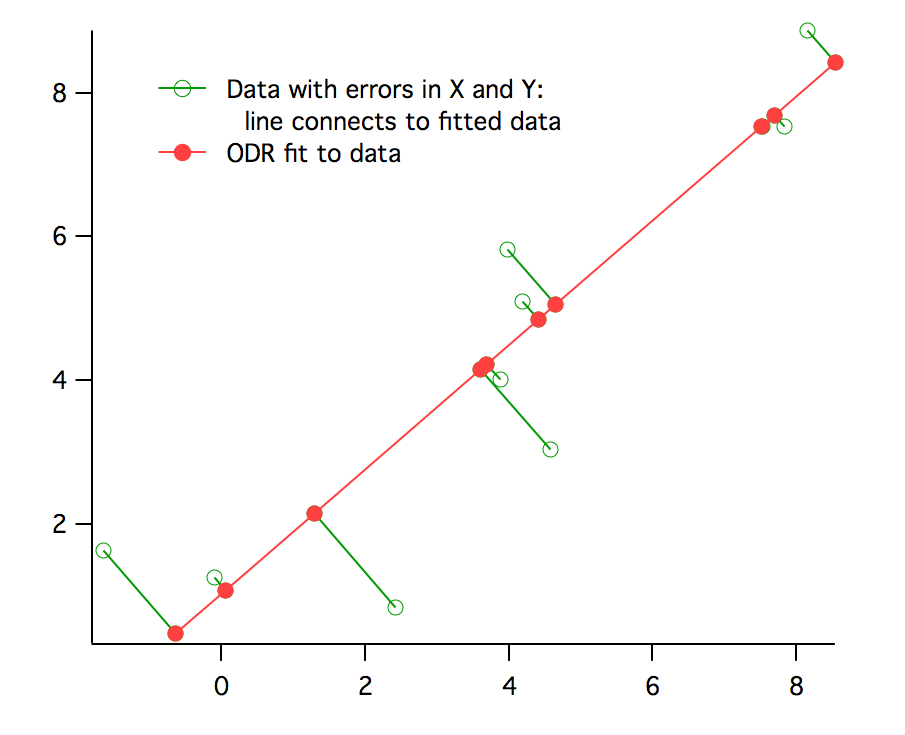
\includegraphics[scale=0.6]{bab4/odr_fit.png}
    \caption{ODR \textit{Fitting}.}
    \label{fig:Ch04_odr}
\end{figure}
ODR menentukan persamaan garis dengan meminimalkan jarak titik ke persamaan garis. Persamaan garis yang diregresi pada \capstone\ ini merupakan persamaan garis lurus yang ditampilkan pada persamaan \ref{eq:garis_lurus}.
\begin{equation}
    \label{eq:garis_lurus}
    y=mx+b
\end{equation}
kemudian garis tegak lurus dicari dengan memberi nilai gradien baru $-\frac{1}{m}$ kemudian dicari titik pada data $(x_0,y_0)$ data dan dibuat persamaan garis yang melalui data dengan gradien tegak lurus seperti yang terlihat pada persamaan \ref{eq:garis_tegak_lurus}.
\begin{equation}
    \label{eq:garis_tegak_lurus}
    y=-\frac{x}{m}+(\frac{x_0}{m}+y_0)
\end{equation}
Koordinat perpotongan garis regresi dengan persamaan garis tegak lurus dapat dicari dengan persamaan \ref*{eqn:ODR}.
\begin{equation}
    \label{eqn:ODR}
    \begin{gathered}
        x_i = \frac{(x_0 + my_0 - m*b)}{(m^2 + 1)}\\
        y_i = m*y_i + b       
    \end{gathered}
\end{equation}
Langkah selanjutnya setelah menemukan titik potong $(x_i,y_i)$ adalah mencari jarak dengan titik $(x_0,y_0)$ pada data hasil bacaan. Persamaan garis diregresi hingga menghasilkan nilai jarak paling minimum dari total titik-titik yang termasuk area garis tersebut.

% https://www.geeksforgeeks.org/orthogonal-distance-regression-using-scipy/

Identifikasi bentuk lingkaran pada data dilakukan dengan metode \textit{Least-square}\cite{d2}. %https://scipy-cookbook.readthedocs.io/items/Least_Squares_Circle.html
Sekelompok titik yang terletak pada $\glsadd{lokasi_r2}\mathbb{R}^2$ dapat dikatakan sebagai  $ \{(x_i,y_i)|0 \leq i \leq N\}$ dengan
$0\leq i \leq N$ menunjukkan data dari 0 hingga $N$. Titik-titik ini digunakan untuk mencari bentuk lingkaran yang paling sesuai untuk mewakilinya yang dituliskan sebagai persamaan \ref*{eqn:Circle} dengan $(x_c\glsadd{x_c},y_c\glsadd{y_c})$ sebagai koordinat pusat lingkaran dan $R$ sebagai jari-jari lingkaran. 
\begin{equation}
    \label{eqn:Circle}
    (x-x_c)^2+(y-y_c)^2+R^2=0
\end{equation}
Langkah pertama \textit{circle fitting} adalah dengan mengasumsikan nilai baru $u$ dan $v$ menjadi:
\begin{equation}
    \begin{gathered}
        u_i=x_i-\bar{x}, \\ 
        v_i=y_i-\bar{y}
        \label{eqn:asumsi_uv}
    \end{gathered} 
\end{equation}

 \begin{tabbing}
dengan: \=\\
    \>$i$ \qquad \qquad \qquad \=: menunjukkan titik ke-$i$,\\ 
    \>$\bar{x}=\frac{1}{N}\sum_{i=1}^n x_i$      \>: nilai rata-rata titik $x$ dari titik pertama hingga titik terakhir $n$,\\
    \>$\bar{y}=\frac{1}{N}\sum_{i=1}^n y_i$      \>: nilai rata-rata titik $y$ dari titik pertama hingga titik terakhir $n$.
 \end{tabbing}
%  $\bar{x}=\frac{1}{N}\sum_i x_i$ dan $\bar{y}=\frac{1}{N}\sum_i y_i$ merupakan rata-rata nilai $x$ dan $y$.
% rumus circle fitting AllahuAkbar:
% Given a finite set of points in $\glsadd{lokasi_r2}\mathbb{R}^2$ ,say $ \{(x_i,y_i)|0 \leq i \leq N\}$\\
% we estimate the best circle : $(x-x_c\glsadd{x_c})^2+(y-y_c\glsadd{y_c})^2+R^2=0$ define: $\bar{x}=\frac{1}{N}\sum_i x_i$ and $\bar{y}=\frac{1}{N}\sum_i y_i$
% dengan $u_i=x_i-\bar{x}, v_i=y_i-\bar{y}\ for\ 0\leq i \leq N$ 
% We solve the problem first in (u, v) coordinates, and then transform back to (x, y)\\
Persamaan diselesaikan dalam koordinat $(u,v)$ dan kemudian dikembalikan ke koordinat $(x,y)$. Lingkaran baru memiliki koordinat titik tengah $(u_c, v_c)$ dan jari-jari $R$, maka nilai yang ingin diminimalkan adalah:
\begin{equation}
    \begin{gathered}
        S=\sum_{i=1}^n ((u_i-u_c)^2+(v_i-v_c)^2+\alpha)^2\\
        \alpha=R^2
        \label{eqn:yang_diminimalkan}
    \end{gathered} 
\end{equation}
dengan nilai $S$ merupakan jarak titik $(u_i, v_i)$ dengan lingkaran. Hal tersebut dapat dicapai dengan melakukan diferensial pada $S(\alpha, u_c, v_c)$. Permasalahan kemudian diselesaikan dengan memberi nilai diferensial setiap parameter menjadi:
\begin{equation}
    \begin{gathered}
        \frac{\partial S}{\partial \alpha} =0,\\ 
        \frac{\partial S}{\partial u_c} =0,\\
        \frac{\partial S}{\partial v_c} =0
        \label{eqn:yang_diferensial}
    \end{gathered} 
\end{equation}
sehingga menghasilkan persamaan yang tertulis pada persamaan \ref*{eqn:turunan1}, \ref*{eqn:turunan2}, dan \ref*{eqn:turunan3}.

\begin{align}
    \label{eqn:turunan1}
    \sum_{i=1}^n ((u_i-u_c)^2+(v_i-v_c)^2-\alpha)=0, \\
    \label{eqn:turunan2}
    \sum_{i=1}^n u_i((u_i-u_c)^2+(v_i-v_c)^2-\alpha)=0, \\
    \label{eqn:turunan3}
    \sum_{i=1}^n v_i((u_i-u_c)^2+(v_i-v_c)^2-\alpha)=0.
\end{align}

% Let the circle have center  and radius R. We want to minimize $S=\sum_i (g(u_i,v_i))^2$  $g(u,v)=(u-u_c)^2+(v-v_c)^2+\alpha$  $\alpha=R^2$\\. 
% To do that, we differentiate $S(\alpha, u_c, v_c).$\\
% this problem is solved by setting the derivation of each parameter to zero: $\frac{\partial S}{\partial \alpha} =0, \frac{\partial S}{\partial u_c} =0, and \frac{\partial S}{\partial v_c} =0 $ sehingga:\\
% $
% \sum_i=1^n ((u_i-u_c)^2+(v_i-v_c)^2-\alpha)=0, \newline
% \sum_i=1^n u_i((u_i-u_c)^2+(v_i-v_c)^2-\alpha)=0, \newline
% \sum_i=1^n v_i((u_i-u_c)^2+(v_i-v_c)^2-\alpha)=0,
% $
Pusat lingkaran dapat diperoleh dengan menyelesaikan persamaan \ref*{eqn:turunan2} dan \ref*{eqn:turunan3} yang menghasilkan persamaan \ref*{eqn:pusat_uv} dan \ref*{eqn:pusat_uv2}.
\begin{align}
    \label{eqn:pusat_uv}
    u_c=\frac{S_{uuv}S_{uv}-S_{uuu}S_{vv}-S_{uvv}S_{vv}+S_{uv}S_{vvv}}{2(S^2_{uv}-S_{uu}S_{vv})}\\
    \label{eqn:pusat_uv2}
    v_c=\frac{-S_{uu}S_{uuv}-S_{uuu}S_{uv}-S_{uv}S_{uvv}+S_{uu}S_{vvv}}{2(S^2_{uv}-S_{uu}S_{vv})}.
\end{align}
\begin{tabbing}
    dengan \=variabel-variabel baru yang didefinisikan sebagai berikut:\\
    
    \>$S_u = \sum_{i=1}^n u_i$,\\
    \>$Sv = \sum_{i=1}^n v_i$,\\
    \>$S_{uu} = \sum_{i=1}^n u_i^2$,\\
    \>$S_{vv} = \sum_{i=1}^n v_i^2$,\\
    \>$S_{uv} = \sum_{i=1}^n u_i v_i$,\\
    \>$S_{uuu} = \sum_{i=1}^n u_i^3$,\\
    \>$S_{vvv} = \sum_{i=1}^n v_i^3$,\\
    \>$S_{uvv} = \sum_{i=1}^n u_i v_i^2$,\\
    \>$S_{vuu} = \sum_{i=1}^n v_i u_i^2$.
\end{tabbing}
% can be rewritten like:
% $S_{uuu} - 2u_c S_{uu}+u_c^2S_u+S_{uvv}-2v_cS_{uv}+v_c^2S_u-\alpha S_u=0$\\
% $S_u=0,$ maka simplify:
% $\\ u_cS_{uu}+v_c S_{uv}=\frac{1}{2}(S_{uuu}+S_{uvv})$\\
%
% $S_v=0,$ maka simplify:
% $\\ u_cS_{uv}+v_c S_{uv}=\frac{1}{2}(S_{vvv}+S_{vuu})$\\
% jadi 
% $
% u_c=\frac{S_{uuv}S_{uv}-S_{uuu}S_{vv}-S_{uvv}S_{vv}+S_{uv}S_{vvv}}{2(S^2_{uv}-S_{uu}S_{vv})}\\
% v_c=\frac{-S_{uu}S_{uuv}-S_{uuu}S_{uv}-S_{uv}S_{uvv}+S_{uu}S_{vvv}}{2(S^2_{uv}-S_{uu}S_{vv})}\\
% $
Radius lingkaran $(u_c, v_c)^T$ akhirnya dapat diperoleh ketika $S_{uuu}S_{vu}-S^2_{uv} \neq 0,$ persamaan dibawa kembali ke koordinat $(x,y)$ sehingga nilai titik pusat $(x_c\glsadd{x_c},y_c\glsadd{y_c})$ dan radius lingkaran ($R$) dituliskan sebagai berikut:
\begin{align}
    \label{eqn:final_circle_equation}
    (x_c\glsadd{x_c},y_c\glsadd{y_c})^T=(u_c,v_c)^T+(\bar{x},\bar{y})^T\\
    R=\sqrt{\alpha}=\sqrt{u_c^2+v_c^2+\frac{S_{uu}+S_{vv}}{n}}.
\end{align}

\subsection{Klasifikasi Manusia}
\label{sec:Klasifikasi}

Langkah terakhir adalah mengidentifikasi keberadaan manusia dari segmen-segmen lingkaran yang telah terbaca. Klasifikasi manusia dilakukan dengan menganalisis segmen lingkaran yang ditemukan pada denah, kemudian lingkaran-lingkaran yang berbentuk mirip kaki manusia akan dianggap sebagai kaki. Posisi manusia nantinya akan ditandai dengan area sepasang kaki berdiri. Sepasang kaki yang memenuhi syarat akan ditampilkan dengan bingkai  segi empat berwarna merah. Cara kerja program deteksi manusia terlihat pada algoritma \ref*{algo:deteksi}.

\begin{algorithm}[H]
    \caption{People Detection} 
    \label{algo:deteksi}
    \begin{algorithmic}[1]
        \Require $\textbf{circle}$ (leg candidates), $\textbf{N}_{circle}$ (the number of leg candidates), $\textbf{N}_{leg}$ (the number of legs), $\textbf{counter}_{person}$
        \For{$i=1 \to \textbf{N}_{circle}$} 
            \If{$\textbf{r}_{circle[i]}<10$}
                    \If{$\textbf{r}_{circle[i+1]}<10$}
                        \State $circle[i] \to leg$ add new data
                        \State $circle[i+1] \to leg[i+1]$ add new data
                    \Else
                        \State continue
                    \EndIf
            \Else
                \State continue
            \EndIf
        \EndFor
        \For{$i=1 \to \textbf{N}_{leg}$}
                \If{distance$(leg[i],leg[i+1])<50$ cm}
                \State $counter_{person}+1$
                \State $people_{data} \gets leg[i],leg[i+1]$
                \Else
                \State continue
                \EndIf
        \EndFor
    \State \Return People and legs position data set
    \end{algorithmic}
\end{algorithm}

Lingkaran pertama yang terdeteksi harus memenuhi kriteria ukuran untuk dikategorikan sebagai kaki manusia, setelah itu dicari lingkaran kedua yang memenuhi kategori tersebut. Langkah terakhir yaitu mencatat jarak antara kedua lingkaran yang ditemukan, apabila jarak kurang dari 50 cm maka kedua lingkaran tersebut dianggap sebagai posisi manusia berdiri. Proses klasifikasi terus diulang-ulang untuk semua lingkaran yang terdeteksi.

\begin{figure}[H]
    \centering
    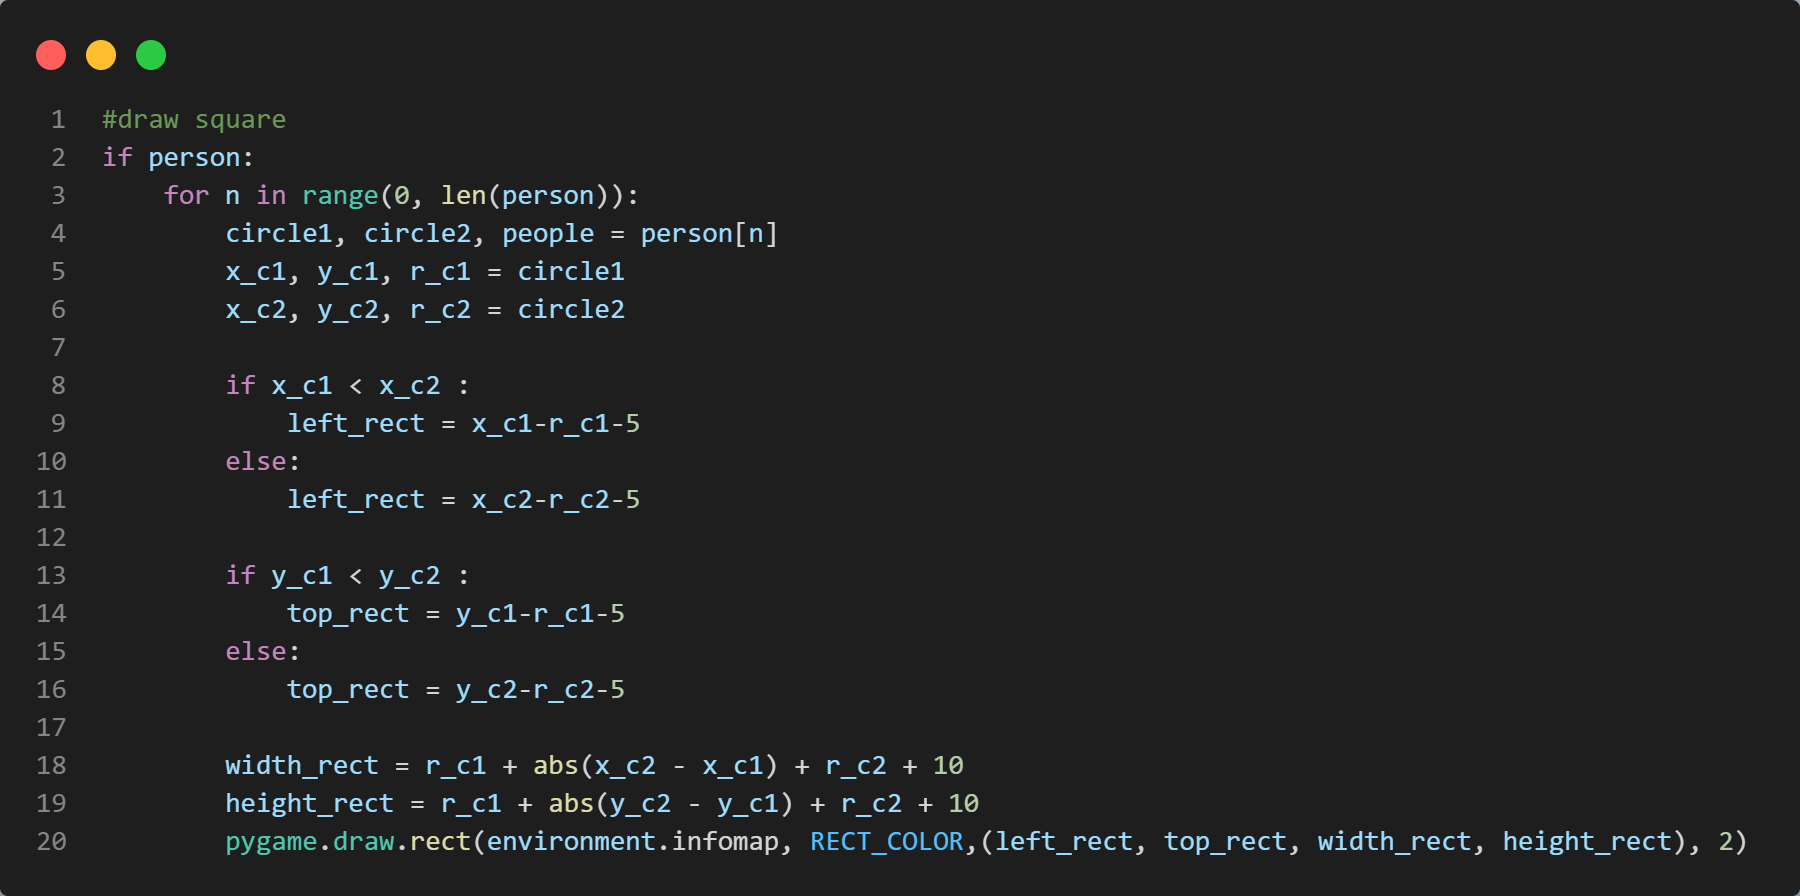
\includegraphics[width=\textwidth]{snippet/klasifikasi_manusia.png}
    \caption{Potongan Program Klasifikasi Manusia.}
    \label{fig:Ch04_klasifikasi_manusia}
\end{figure}

Potongan program pada Gambar \ref*{fig:Ch04_klasifikasi_manusia} menunjukkan proses pemberian bingkai  segi empat untuk sepasang kaki manusia yang terdeteksi. Program ini hanya berjalan jika manusia sudah dipastikan ada dalam denah pada program sebelumnya. Baris program nomor 4,5,6 berfungsi untuk ekstraksi variabel-variabel pada kedua kaki manusia. Variabel dipisah menjadi $x_c\glsadd{x_c},y_c\glsadd{y_c}$ yang menunjukkan koordinat pusat lingkaran masing-masing kaki dan $r_c\glsadd{r_c}$ yang menunjukkan radius masing-masing kaki. Baris 8 hingga 16 digunakan untuk menghitung batas kiri dan batas atas bingkai segi empat. Batas dihitung dengan menambahkan $5$ cm dari titik terluar sepasang kaki. Batas dikembangkan menjadi segi empat kemudian ditampilkan pada simulasi \textit{pygame}.

\section{\textit{Improvement}}
\label{sec:improvement}
Sistem yang dirancang sebelumnya tidak dapat langsung diterapkan, algoritma yang diadopsi sistem memerlukan beberapa perubahan pada beberapa tahap pendeteksian. Algoritma \textit{seed-growing} yang tertulis pada bab sebelumnya hanya berfungsi untuk mendeteksi adanya satu bentuk garis dalam satu kali pemindaian \lidar\ yaitu garis lurus. Algoritma \textit{seed-growing} perlu ditulis ulang untuk dapat mengaplikasikan pemindaian lingkaran. Pada bab ini dituliskan algoritma hasil \textit{improvement} yang khusus diterapkan untuk pemindaian segmen lingkaran dari hasil bacaan mentah sensor.

\begin{algorithm}[H]
    \caption{New Seed-segment Detection} 
    \label{algo:algo3}
    \begin{algorithmic}[1]
        \Require $\textbf{N}_{p}\glsadd{N_p},\epsilon\glsadd{epsilon}, \glsadd{delta}\delta, \glsadd{Snum}S_{num}, \glsadd{Pmin}P_{min}$  
        \State Initialization flag = true
        \For {$i=1 \to (\textbf{N}_{p}\glsadd{N_p}-\textbf{P}_{min})$}
            \State $j \gets i + \textbf{S}_{num}$
            \State fit \glsadd{segmen}\textbf{Seed}$(i,j)$
            \For {$k=i \to j$}
                \State \hl{flag = true}
                \State obtain the predicted point or the next point $P'_{k}$
                \State $d_{1} \gets distance\ from\ P_{k}\ to\ P'_{k}$
                \If{$d_{1}>\glsadd{delta}\delta$}
                    \State $flag=false$
                    \State break
                \EndIf
                \State $d_{2}\gets distance\ from\ P_{k}\ to\ \glsadd{segmen}\textbf{Seed} (i,j)$
                \If{$d_{2}>\epsilon\glsadd{epsilon}$}
                    \State $flag = false$
                    \State break
                \EndIf 
            \EndFor
            \If{$flag==true$}
                \State return $\glsadd{segmen}\textbf{Seed} (i,j)$
            \EndIf
        \EndFor
    \end{algorithmic} 
\end{algorithm}

Perubahan pertama dilakukan pada algoritma \textit{seed detection} dengan penambahan nilai variabel. Terlihat pada algoritma \ref*{algo:algo3} bahwa pada baris enam perlu ditambah nilai \textit{true} pada variabel \textit{flag} agar sistem berhasil mendeteksi lebih dari satu segmen dalam satu putaran pembacaan \lidar. Algoritma sebelumnya akan menghentikan proses pencarian segmen ketika sudah ditemukan satu \textit{seed-segment}. Perubahan ini membuat sistem lebih mudah menghitung banyak objek lingkaran di sekitar robot yang dideteksi.

\begin{algorithm}[H]
    \caption{Circle Segment Region Growing} 
    \label{algo:algo4}
    \begin{algorithmic}[1]
        \Require $\glsadd{segmen}\textbf{Seed} (i,j),\textbf{N}_{p}\glsadd{N_p}, \textbf{P}_{min}, \textbf{L}_{min}, \epsilon\glsadd{epsilon}$ 
        \State Initialization: $\textbf{Line}(P_{b},P_{f})\gets \glsadd{segmen}\textbf{Seed} (i,j),\textbf{L}_{l}=0, \textbf{P}_{l}=0 $
        \State $\textbf{P}_{f}=j+1, \textbf{P}_{b}=i-1$
        \While{$\textbf{P}_{f}<\textbf{N}_{p}\glsadd{N_p}$}
            \If{\hl{$distance(\textbf{P}_{f},\textbf{P}_{f-1})<\glsadd{delta}\delta$}}
                \If{\hl{$distance(circle,\textbf{P}_{f})<\epsilon\glsadd{epsilon}$}}
                    \State refit $\textbf{Line}(\textbf{P}_{b}, \textbf{P}_{f})$
                    \State $P_{f} \gets P_{f}+1$
                \Else
                    \State break
                \EndIf
            \Else
                \State break
            \EndIf
            \State $P_{f} \gets P_{f}-1$
        \EndWhile

        \While{$\textbf{P}_{b}>0$}
            \If{\hl{$distance(\textbf{P}_{b},\textbf{P}_{b+1})<\glsadd{delta}\delta$}}
                \If{\hl{$distance(circle,\textbf{P}_{b})<\epsilon\glsadd{epsilon}$}}
                    \State refit $\textbf{Line}(\textbf{P}_{b}, \textbf{P}_{b})$
                    \State $P_{b} \gets P_{b}-1$
                \Else
                    \State break
                \EndIf
            \Else
                \State break
            \EndIf
            \State $P_{b} \gets P_{b}+1$
        \EndWhile
        \State $P_{b} \gets P_{b}+1$
        \State obtain $\textbf{L}_{l}, \textbf{P}_{l}$ from $\textbf{Line}(\textbf{P}_{b}, \textbf{P}_{f})$
        \If{$(\textbf{L}_{l} \geq \textbf{L}_{min}) \& (\textbf{P}_{l} \geq \textbf{P}_{min})$}
            \State \Return $\textbf{Line}(\textbf{P}_{b}, \textbf{P}_{f})$ with $\textbf{Parameters}(a,b,c)$
        \EndIf

    \end{algorithmic}
\end{algorithm}

Pendeteksian segmen utuh lingkaran juga memerlukan perubahan menjadi sedikit berbeda dengan segmen garis. Perubahan yang dilakukan dapat dilihat pada algoritma \ref*{algo:algo4}. Perubahan dilakukan pada urutan peninjauan jarak antar titik dengan jarak titik dan lingkaran. Pada algoritma awal, titik akan ditinjau dari jarak titik terhadap persamaan garis yang ada terlebih dahulu. Hal ini membuat program gagal mengidentifikasi segmen lingkaran karena membuat segmen tidak bisa berkembang. Hal ini disebabkan oleh sedikitnya jumlah titik sehingga jari-jari yang terdeteksi hanya berukuran kecil tidak sesuai dengan jari-jari lingkaran sesungguhnya sehingga ketika dihitung jarak titik dengan lingkaran maka menghasilkan angka yang terlalu besar hingga menghentikan proses pencarian. Penggantian urutan perhitungan jarak ini membuat sistem berhasil menemukan segmen yang lebih utuh mendekati bentuk lingkaran aslinya.

Kedua algoritma baru ini diperlukan untuk diterapkan bersama algoritma sebelumnya agar meningkatkan keberhasilan sistem deteksi. Algoritma baru tersebut menghilangkan kekurangan algoritma sebelumnya yang tidak dapat mendeteksi dan menyimpan data segmen-segmen yang dibaca dalam satu kali pemindaian. Penyimpanan data-data segmen yang terdeteksi merupakan langkah penting untuk mendeteksi sepasang lingkaran menjadi kandidat kaki manusia. Adanya perubahan ini membuat sistem bisa melanjutkan proses deteksi kaki manusia.



